\documentclass[11pt,a4paper]{extarticle}
\usepackage{cmap}
\usepackage[utf8x]{inputenc}
\usepackage[T2A,T1]{fontenc}
\usepackage[english,russian]{babel}
\usepackage[hidelinks]{hyperref}
\usepackage{hyperref}
\usepackage[nottoc,numbib]{tocbibind}
\usepackage{listings,lstautogobble}
\usepackage{amsthm}
\usepackage{amsmath}
\usepackage{amsfonts}
\usepackage{amssymb}
\usepackage{cite}
\usepackage{xcolor,colortbl}
\usepackage{graphicx}
\usepackage{mathtools}
\usepackage{subcaption}
\usepackage{enumerate}
\usepackage{minted}
\usepackage{perpage}
\usepackage{subcaption}
\usepackage{pythonhighlight}
\usepackage{fullpage}

\definecolor{Gray}{gray}{0.95}
\definecolor{Red}{rgb}{0.80,0.5,0.5}
\definecolor{Green}{rgb}{0.6,0.8,0.6}
\definecolor{monokaibg}{HTML}{272822}

\usemintedstyle{pastie}
% \setminted{bgcolor=monokaibg}
\setminted{fontsize=\small}

\definecolor{Gray}{gray}{0.95}
\definecolor{Black}{gray}{0.1}
\definecolor{Red}{rgb}{0.80,0.5,0.5}
\definecolor{Green}{rgb}{0.6,0.8,0.6}

\definecolor{codegray}{rgb}{0.5,0.5,0.5}
\definecolor{codepurple}{rgb}{0.58,0,0.82}
\definecolor{backcolour}{rgb}{0.95,0.95,0.92}

\newlength{\twosubht}
\newsavebox{\twosubbox}
\setlength\headheight{26pt}

\newenvironment{compactlist}{
\begin{list}{{$\bullet$}}{
\setlength\partopsep{0pt}
\setlength\parskip{0pt}
\setlength\parsep{0pt}
\setlength\topsep{0pt}
\setlength\itemsep{0pt}
}}{
\end{list}
}
\providecommand\phantomsection{}
\MakePerPage{footnote}
% \renewcommand{\baselinestretch}{1.2}

\begin{document}
\selectlanguage{russian}
\begin{titlepage}
	\begin{centering}
		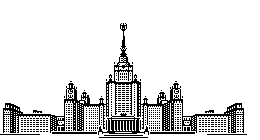
\includegraphics{img/msu}\\
		\large{
			\textbf{Московский государственный университет имени М.В. Ломоносова}\\
			Факультет вычислительной математики и кибернетики\\
			Кафедра интеллектуальных информационных технологий\\
			Лаборатория компьютерной графики и мультимедиа\\[4cm]
		}
		\Large{
			Гончаренко Дмитрий Александрович\\[0.9cm]
		}
		\Large{
			\textbf{Алгоритм изменения времени суток на изображении}\\
			% \textbf{Research of Changing The Time of Day on Images}\\
		}
		\rule[0.3cm]{14cm}{0.02cm}\\[1cm]
		\large{
			ВЫПУСКНАЯ КВАЛИФИКАЦИОННАЯ РАБОТА\\[4cm]
		}
	\end{centering}
	\begin{flushright}
		\large{
			\textbf{Научный руководитель:}\\ К.С. Зипа\\
		}
	\end{flushright}
	\begin{center}
		\vfill
		\large{
			Москва, 2019
		}
	\end{center}
\end{titlepage}

\begin{abstract}
	Алгоритм изменения времени суток на изображении относится к классу задач машинного обучения по \textit{переносу
	изображений}\footnote{
		\textbf{Перенос изображений} (англ. \textit{image translation}, или \textit{image transfering})
		-- подвид технологии переноса обучения, позволяющий сохранять и объединять извлеченные признаки изображений.
	}.
	Данная сфера значительное продвинулась благодаря современным вычислительным возможностям, в частности, переносе обучения на графические процессоры, GPU.
	За последние несколько лет появилось немало исследовательских работ на тему междоменных переносов изображений, стилей и колоризации.
	В данной работе рассматриваются современные подходы к переносу изображений, применимые к задаче изменения времени суток на изображении.
	Проводится описание нейросетевых моделей, обоснование и выбор метода и сравнительный анализ серии экспериментов обучения.
\end{abstract}

\selectlanguage{english}
\begin{abstract}
	The algorithm of changing the time of the day on images is a subclass of Machine Learning problems of image translation.
	This area has advanced significantly due to the modern computing capabilities, in particular the training transfer on GPUs.
	Over the past few years, many research papers have appeared on the subjects of crossdomain images translation, styles transfering and colorization.
	This research reveals modern approaches of image translation applicable to problem of changing the time of day on the image.
	A description of the neural network models, the rationale and choice of method for training, and a comparative quality analysis of a series of training experiments are carried out.
\end{abstract}
\selectlanguage{russian}

\newpage
\tableofcontents
\newpage

\section{Введение}

	Многие математические описания моделей машинного обучения появились еще в середине 20-го века.
	А в конце 50х годов уже начались первые попытки их практической реализации.
	Спустя почти полвека задачи машинного обучения все также не теряют своей актуальности.
	Рост числа работ, открытие исследовательских центров внутри компаний и при университетах показывает,
	что высокий интерес к данной сфере не ограничивается только наукой.
	За последние 10 лет появилось множество удобных инструментов для построения самых разнообразных моделей обучения, что оказало немалое влияние на развитие \textit{науки о данных}\footnote{
		\textbf{Наука о данных} (англ. \textit{data science}) -- соовокупность процессов и методов направленных на извлечение информации из исследуемых данных.
	}.  
	
	Стоит отметить, что не последнюю роль здесь сыграли многократно выросшие вычислительные возможности. 
	Это позволило обучать \textit{нейронные сети}\footnote{
		\textbf{Нейронная сеть} --  математическая модель, а также её программное или аппаратное воплощение, 
		построенная по принципу организации и функционирования биологических нейронных сетей -- сетей нервных клеток живого организма.
		Является мощным современным инструментом машинного обучения.
		Главная особенность -- способность обучаться на предоставленных данных, называемых тренировочными.
		Помимо исследовательских направлений нейронные сети также активно используются в комерции, например обработка спама на электронной почте или система рекомендаций в интернет-магазинах.
	} на персональных компьютерах за несколько минут, для чего ранее могли требоваться недели, а то и месяцы на специализированных вычислительных устройствах.

	\textit{Перенос обучения} является одной из центральных исследовательских задач современного машинного обучения.
	Данная область направленна на получение некоторой информации об объекте, сохранение и последующее применение этих знаний к другому объекту, связанному с первым.   
	\textit{Перенос изображений}, в свою очередь, является подклассом переноса обучения применяемым на изображениях. 
	В настоящее время переносу изображений уделяется значительное внимание в исследовательских работах~\cite{i2ipapers}, а разнообразие сферы применения поистине впечатляющее.
	Так с помощью переноса изображений можно добиться объединения стилей двух изображений~\cite{style_transfer}, что может использоваться художниками в создании интересных картин и композиций,
	колоризации\footnote{ \textbf{Колоризация} (англ. \textit{colorization}) -- преобразование монохромных изображений в цветные.} черно-белых фотографий~\cite{color_transfer},
	благодаря чему можно в автоматизированном режиме перекрашивать отцифрованные монохромные киноленты и фотоснимки,
	объединение локальных признаков объектов и животных~\cite{CycleGAN}, что позволяет создавать несуществующие породы животных и по наброску генерировать текстурированное изображение,
	увеличение разрешения изображений~\cite{super_resolution}, с помощью чего можно достигать точности, превышающей традиционные алгоритмы билинейной интерполяции.

	В данной исследовательской работе рассматриваются и систематизируются современные подходы переноса изображений, применимые к задаче изменения времени суток на изображениях.
	Проводится обучение подходящего алгоритма на различных наборах тренировочных данных.
	Моя задача состоит в получении предобученной модели, умеющей из изображений дня синтезировать реалистичные изображения ночи,
	и наоборот из ночи научиться генерировать максимально правдоподобное изображение дня. 
	Также я провожу сравнительный анализ скорости переноса и качества полученных результатов.
	
	В качестве инструмента был выбран фреймворк PyTorch\footnote{
		\textbf{PyTorch} -- библиотека машинного обучения, основанная на Torch. Разработана исследовательской группой в Facebook.
	}, так как он разработан в виде библиотеки для языка Python -- основного языка современного машинного обучения~\cite{ml_lang},
	и зарекомендовал себя мощным и гибким инструментом для исследования и обучения нейронных сетей.


\newpage
\section{Постановка задачи}
	% \subsection{Актуальность задачи}
	% 	Решение задачи изменения времени суток можно использовать в проектировании создании 3D моделей и макетов,
	% 	не будет необходимости перирисовывать и видоизменять модель для ночной сцены, если уже создана дневная.
	% 	для видеоиграх, для смены времени сцены, в рекламе.


	\subsection{Цель работы}

		В науке о данных одну из ключевых ролей играет непосредственный выбор данных, на которых будет обучаться сеть, 
		и которые будут использоваться для валидации качества модели. Перенос изображений не является исключением.
		Цель работы -- получить модель, которая будет уметь переносить изображения между \textit{доменами}\footnote{
			\textbf{Домен} -- область, множество, содержащее в себе объекты одного типа. 
		} дня и ночи и будет способна с высокой точностью решить проблему изменения времени суток на изображениях.


	\subsection{Решаемые задачи}

		Проблему изменения времени суток на изображении можно разбить на следующие этапы:
		\newline
		\begin{itemize}
			\vspace{-1em}
			\item Исследование существующих методов переноса изображений и анализ решений родственных задач
			\item Поиск применимых к проблеме тренировочных данных -- изображений с различными временем суток
			\item Классификация тренировочных данных и перенос изображений по доменам 
			\item На основе проведенного исследования и обзора литературы, выбор модели, подходящей для решения поставленной задачи
			наилучшим образом
			\item Множественное обучение выбранной модели с различными конфигурациями на наборах данных с помощью библиотеки PyTorch
			\item Проведение серии экспериментов переноса изображений для получения оценки качества и скорости работы модели 
		\end{itemize}


	\subsection{Формальная постановка задачи}\label{intro_problem}

		Формально алгоритм изменения времени суток на изображении можно сформулировать следующим образом:
		\vspace{-1em}
		\subsubsection*{Вход}
			На вход алгоритму поступают два изображения из различных доменов \(x_{1} \in X_{1}\)  и \(x_{2}\ \in X_{2}\), где
			\begin{itemize}
				\item \(X_{1}\) -- домен с набором изображений первого типа
				\item \(X_{2}\) -- домен с набором изображений второго типа
			\end{itemize}
			Не ограничивая общности, пусть \(X_{1}\) соодержит изображения дня, а \(X_{2}\) соответвует ночи.
		\vspace{-1em}
		\subsubsection*{Выход}
			Необходимо построить \textit{кросдоменные}\footnote{
				\textbf{Кросдоменный перенос} (англ. \textit{cross-domain transfer}) -- перенос объектов между доменами 
			} отображения \(f_{12}\!: X_{1} \longrightarrow X_{2}\) и \(f_{21}\!: X_{2} \longrightarrow X_{1}\).
			
			\noindent
			Реализовать функцию, принимающую на вход изображения из разных доменов
			\(x_{1}, x_{2}\) и возвращающую перенесенные изображения \(x_{2}', x_{1}'\) соответственно: 

			\begin{equation}
				x_{2}', x_{1}' = CrossDomainTranslator(x_{1}, x_{2}),\ \text{где}\ x_{1}' \in X_{1},\ x_{2}' \in X_{2}
			\end{equation}
	

\newpage
\section{Обзор существующих методов}
	
	На сегодняшний день одними из наиболее популярных алгоритмов, на которых базируются решения многих задач переноса изображений, являются
	генеративно состязательные нейронные сети и вариационные автоэнкодеры.
	В этой главе я исследую подходы решения родственных методов и обосновываю выбор алгоритма для выполнения поставленной задачи. 


	\subsection{Генеративно состязательные сети (GAN)}		

		\textbf{Генеративно состязательная нейронная сеть} (GAN) -- комбинация двух нейронных сетей $G$ (генератор) и $D$ (дискриминатор).
		Генератор подбирает \textit{латентные}\footnote{
			\textbf{Латентный} здесь и далее, то же что и скрытый
		} параметры для генерации нового объекта.
		Дискриминатор пытается отличить оригинал от объекта, созданного генератором.
		
		\begin{figure}[ht]
			\centering
			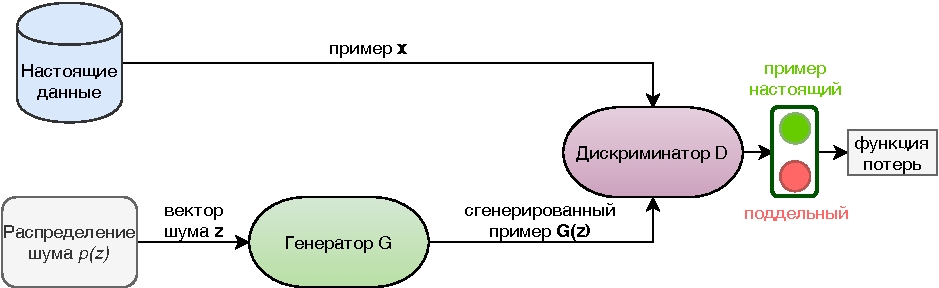
\includegraphics[width=0.8\textwidth]{img/gan}
			\caption{Схема работы генеративно состязательной сети (GAN)}
			\label{pic:gan}
		\end{figure}
		\noindent
		Формально генератор можно определить как отображение некоторого пространства скрытых параметров $\mathcal{Z}$,
		на котором задано априорное распределение \(p_z(z)\), в прострасво данных $\mathcal{X}$.
		Дескриминатор же будет производить отображение $\mathcal{X}$ в отрезок $[0,1]$ -- вероятность того, что пример настоящий.
		На рис.~\ref{pic:gan} представлена общая схема работы генеративной сети.
		\begin{equation}
			\begin{aligned}
				& G\!:{\mathcal{Z}}\rightarrow {\mathcal{X}} \\
				& D\!:{\mathcal{X}}\rightarrow [0,1]
			\end{aligned}
		\end{equation}
		Основной целью генеративно состязательной сети является получение генератором распределения данных $p_{gen}$,
		не отличимого дискриминатором от исходного распределения $p_{data}$.
		То есть, по сути, заключается в решении задачи оптимизации~\cite{Deep_Learning}:
		\begin{equation}\label{eq:gan}
			\min_{G} \max_{D} \mathcal{L}_{\text{\tiny GAN}}(D,G), \text{ где }
		\end{equation}
		\begin{equation*}
			\mathcal{L}_{\text{\tiny GAN}}(D,G) = \mathbb{E}_{x \sim p_{data}(x)}\big[\log{D(x)}\big] + \mathbb{E}_{x \sim p_{z}(z)}\big[\log (1 - D(G(z)))\big]
		\end{equation*}
		\indent


	\subsection{Автокодировщики (AE)}		
	
		\textbf{Автоэнкодер} (AE) -- комбинация двух нейронных сетей: энкодера $E$ (кодировщика) и декодера $D$ (декодировщика).
		Энкодер получает и преобразует данные в сжатый код скрытого пространства.
		Декодер же старается из этого кода восстановить объект наиболее близко к исходному.
		Математически можно представить автоэнкодер как отображения пространства входных данных $\mathcal{X}$ в латентное пространство $\mathcal{Z}$ и обратно:
		\begin{equation}
			\begin{aligned} 
				& E\!:{\mathcal{X}}\rightarrow {\mathcal{Z}} \\
				& D\!:{\mathcal{Z}}\rightarrow {\mathcal{X}} \\
				x& \xrightarrow[]{E} z \xrightarrow[]{D} x', \text{ где }
			\end{aligned}
		\end{equation}
		\begin{equation*}
			\begin{array}{ll}
				x\;\in \mathcal{X}&-\;\text{исходное изображение}\\
				z\;\in \mathcal{Z}&-\;\text{скрытый код}\\
				x' \in \mathcal{X}&-\;\text{восстановленное изображение}\\
			\end{array} 
		\end{equation*}

		\begin{figure}[ht]
			\centering
			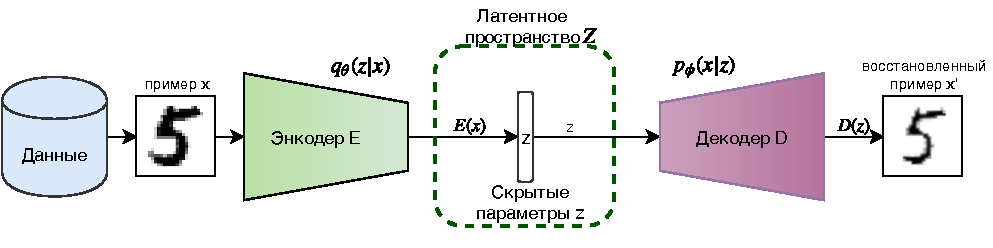
\includegraphics[width=0.8\textwidth]{img/vae}
			\caption{Схема работы вариационных автоэнкодеров (VAE)}
			\label{pic:vae}
		\end{figure}
		\noindent
		Задача автокодировщика состоит в минимизации разницы между исходным изображением $x$ и восстановленным $x'$.
		Для этого вводится функцию потерь $\mathcal{L}_{\text{\tiny AE}}$, характеризующая потери при неправильном принятии решений:
		\begin{equation} \label{eq:ae}
			\mathcal{L}_{\text{\tiny AE}}(x,x') = \|x - x'\|^{2}
		\end{equation}
		Основная проблема автоэнкодеров заключается в том, что скрытое пространство может не быть непрерывным.
		Из-за чего не получается произвести интерполяцию, и как следствие, их область применения ограничивается.
		Эту проблему способны решить вариационные приближения.


	\subsection{Вариационные автокодироващики (VAE)} \label{sec:vae}		

		\textbf{Вариационный автоэнкодер} (VAE) отличается от автоэнкодера непрерывностью латентного пространства
		и предположениями накладываемыми на распределение данных.
		Пусть выбор тренировочных данных $x$ находится в некоторой условной зависимости $p(x|z)$ от переменных скрытого пространства $z$.
		Кодировщик на вход получает пример $x$ и выдает вектор размерности $2d$ распределения скрытых переменных $z$, состоящий из двух векторов размерности $d$:
		вектора стандартных отклонений $\sigma$ и вектора средних значений $\mu$. 
		То есть энкодер представляет собой нейронную сеть с параметрами $\theta$ и обучается апроксимировать апостериорное распределение $q_{\theta}(z|x)$.
		Декодировщик тоже является нейронной сетью с параметрами $\phi$ и старается из вектора размерности $2d$ скрытых переменных $z$ получить объект из вариационного распределения над $x$: $p_{\phi}(x|z)$.
		На рисунке~\ref{pic:vae} представлена верхнеуровневая схема модели вариационных автоэнкодеров.

		Задачей вариационных автоэнкодеров является задача оптимизации~\eqref{eq:vae}.
		Необходимо так подобрать параметры $\theta$ в $q_{\theta}(z|x)$, чтобы максимально точно приблизить $p(z|x)$:
		\begin{equation} \label{eq:vae}
			\arg\min_{\theta} \mathbb{KL}\big(q_{\theta}(z|x)\|p(z|x)\big), \text { где }
		\end{equation}
		\begin{equation*}
			\mathbb{KL}\big(q_{\theta}(z|x)\|p(z|x)\big) = \mathbb{E}_q\big[\log q_{\theta}(z|x)\big] - \mathbb{E}_q\big[\log p(x,z)\big] + \log p(x)
		\end{equation*}
		$\mathbb{KL}$ -- расстояние Кульбака-Лейблера - мера удаленности двух распределений.
		\\\\
		Так или иначе, методы реализующие перенос изображений опираются на состязательные сети GAN, VAE или их модификации.
		Рассмотрим следующие алгоритмы с позиции решения предложенной задачи изменения времени суток на изображении.
		Будем рассматривать, уже введенные в формальном определении, домены изображений \(X_{1}\) и \(X_{2}\), соответствующие разному времени суток (глава~\ref{intro_problem}).
		\\\\Пусть изображения \(x_{1},x_{2}: x_{1} \in X_{1}, x_{2} \in X_{2}\)


	\subsection{Методы использующие обучение с учителем}
	
		\textbf{Обучение с учителем} (англ. \textit{supervised learning}) -- способ машинного обучения, в ходе которого входные данные соотносятся с выходными до начала обучения.
		Обучение происходит на заготовленных парах объектов (\(x_{1},x_{2}\)), называемыми ''стимул-реакция'', которые находятся в доменах в некотором совместном распределении \(P_{X_{1},X_{2}}(x_{1},x_{2})\)\footnote{
			\textbf{Совместное распределение} -- это распределение совместных исходов образованных из нескольких случайных величин.
		}.
		Задача метода -- построить функцию внутренней зависимости между примерами, которая затем будет отображать входные изображения желаемым образом.

		Успешными примерами применения этого способа для решения задач переноса изображения можно считать эти работы~\cite{BicycleGAN, pix2pix}.

		\subsubsection{Условные состязательные сети (cGAN)} \label{sec:pix2pix}

			Метод представленный на международной конференции компьютерного зрения (CVPR) в 2017 году
			исследовательской группой из университета Беркли под именем pix2pix~\cite{pix2pix}
			использует для переноса изображений обучение с учителем и условные генеративно состязательные нейронные сети.

			Условные GAN являются модификацией над стандартными GAN.
			От обычных генеративных сетей~\eqref{eq:gan}, cGAN отличаются добавочным вектором информации $y$ для генератора \(G(z|y)\) и дискриминатора \(D(X|y)\).
			Вектор $y$ может содержать любую уточняющую информацию, например он может содержать метки объектов на изображении,
			в случае c pix2pix, $y$ -- это добавочное входное изображение, видимое генератору и дискриминатору.

			\begin{figure}[ht]
				\centering
				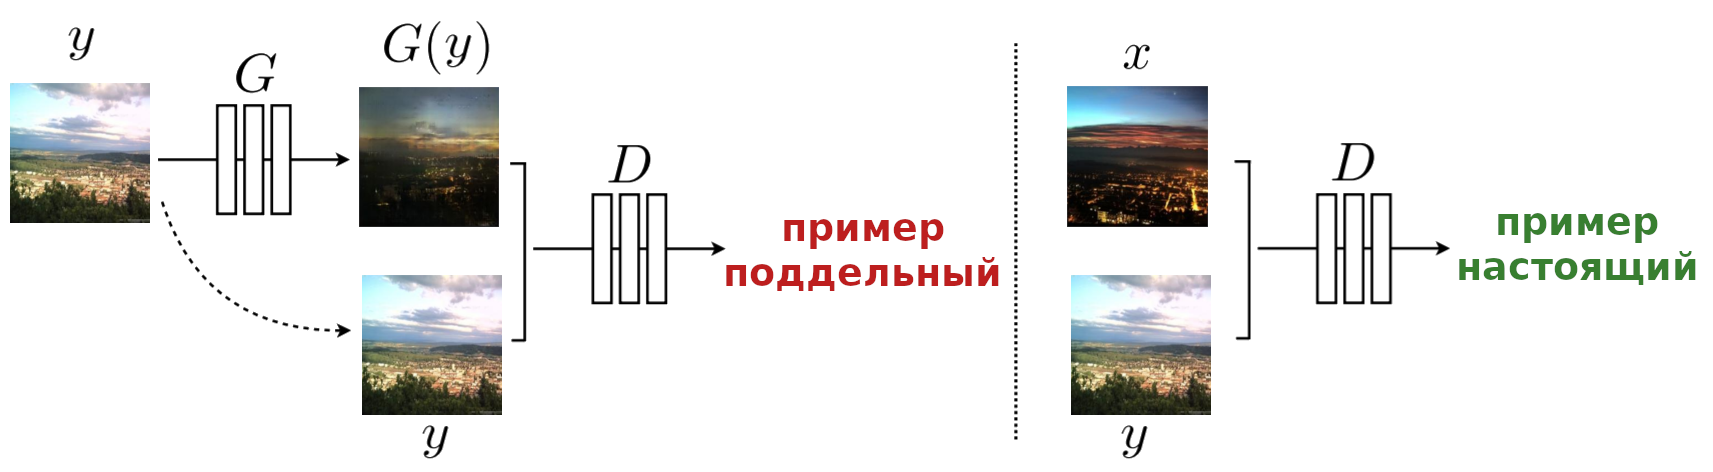
\includegraphics[width=0.9\textwidth]{img/cgan}
				\caption{Схема работы условно генеративно состязательной сети (cGAN)}{
					$x$ -- \emph{настоящее изображение ночи, соответствующее} $y$
				}
				\label{pic:cgan}
			\end{figure}
			\noindent
			Выше на рис.~\ref{pic:cgan} приведена общая схема работы cGAN в модели pix2pix.
			В качестве функции потерь была взята соовокупность двух функций потерь: генеративной сети~\eqref{eq:gan} в случае с cGAN и $\mathcal{L}_1$.
			Сеть решает следующую задачу оптимизации:
			\begin{equation}\label{eq:cgan}
				\arg\min_{G}\max_{D} \Big( \mathcal{L}_{\text{\tiny cGAN}}(D,G) + \lambda \mathcal{L}_1(G) \Big), \text{ где }
			\end{equation}
			\begin{equation*}
					\mathcal{L}_{\text{\tiny cGAN}}(D,G) = \mathbb{E}_{x}\big[\log{D(x)}\big] + \mathbb{E}_{y,z}\big[\log (1 - D(G(z,y)))\big],\;
					\mathcal{L}_1(G) = \sum_{i=1}^{n}\big(x - G(z,y)\big)^2
			\end{equation*}
			$\lambda$ -- параметр, контролирующий вклад $\mathcal{L}_1$.
			При $\lambda = 0$ получаются более четкие изображения, но подверженные артефактам,
			при больших значениях параметра, будут получаться менее четкие, размытые изображения, но с визуально уменьшенным количеством артефактов~\cite{pix2pix}.
			Модель обучалась на датасете\footnote{ \textbf{Датасет} (англ. \textit{dataset}) -- то же, что и набор данных}~\cite{data:paired_night2day}
			парных фотографий (с одинаковых ракурсов) сделанных с уличных вебкамер в разрешении 256x256px в разное время суток.
			После проведения серии экспериментов стало ясно, что на данных, немного отличных от обучающей выборки, точность модели падает,
			появляются артефакты и размытости, поэтому данный метод в своей задаче использовать не получится.
			
			\begin{figure}[ht]
				\centering
				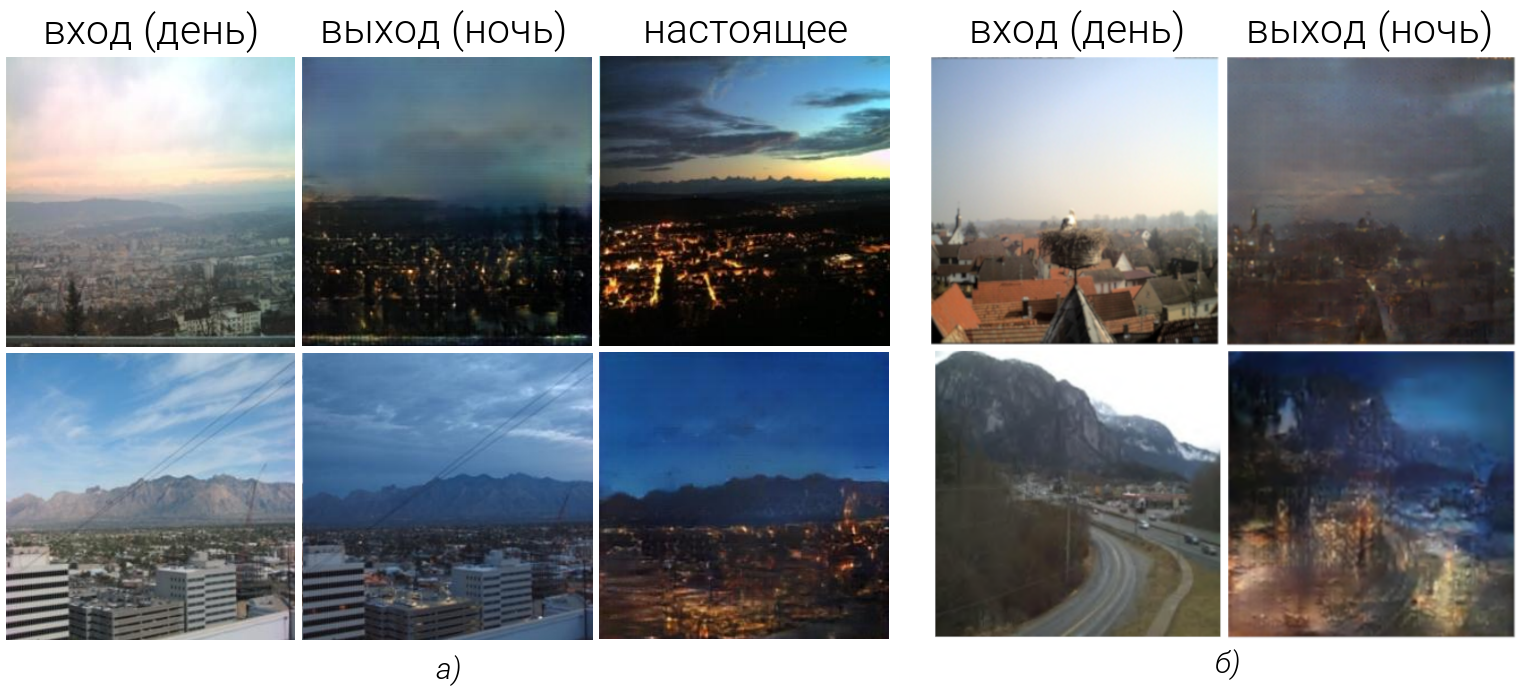
\includegraphics[width=0.85\textwidth]{img/pix2pix_res}
				\caption{Результаты работы pix2pix (день в ночь)}{
					\small{
					(а) успешная работа метода,
					(б) артефакты на нестандартных примерах
				}}
				\label{pic:pix2pix_results}
			\end{figure}
			\noindent
			Резльтаты работы программы изображены на рис.~\ref{pic:pix2pix_results}.
			Как можно видеть~\ref{pic:pix2pix_results} а), метод генерирует довольно неплохие результаты на примерах близких к обучающим,
			но сильно деградирует на нестандартных изображениях, отличных от тренировочной выборки~\ref{pic:pix2pix_results} б). 
			\\\\Существенной проблемой медотов, использующих обучение с учителем, является необходимость хранить объекты доменов по парам.
			Это сказывается на сложности поиска и сбора тренировочных данных для применения их на практике.
			С другой стороны, методы без учителя, лишены этого недостатка, и данные можно получать фактически ''из воздуха''.
			
			
	\subsection{Методы использующие обучение без учителя}

		\textbf{Обучение без учителя} (англ. \textit{unsupervised learning}) -- совокупность задач машинного обучения, решаемых на неразмеченных данных.
		В отличие от обучения с учителем, где тренировочные данные находятся в совместном распределении \(P_{X_{1},X_{2}}(x_{1},x_{2})\), в методах без вмешательства учителя требуется
		найти априорное распределение, выбирая данные (\(x_{1},x_{2}\)) из доменов с частным распределением \(P_{X_{1}}(x_{1})\) и  \(P_{X_{2}}(x_{2})\)\footnote{
			\textbf{Частное распределение} -- это распределение вероятности компонент некоторого множества, без зависимости между компонентами.
		}.

		\noindent
		Метод обучения без учителя значительное упрощает сбор тренировочных данных, так как для обучения не требуются парные объекты.
		К минусам можно отнести, что этот подход требует большего числа обучающих изображений для получения реалистичных результатов, чем методы с учителем.
		К наиболее интересным работам, использующим этот подход, можно отнести~\cite{UNIT,MUNIT,CycleGAN}.
		
		\subsubsection{Цикловая согласованность (CC)}\label{sec:cc}

			Введем новое понятие, которое будет использоваться в алгоритмах обучения без учителя.
			\textbf{Цикловая согласованность} (также \textbf{круговая}, англ. \textit{cycle-consistency}) означает,
			что если изображение перенести между доменами и обратно, то должно получиться исходное изображение.
			Более формально: пусть заданы биективные отображения \(G: X \rightarrow Y\) и \(F: Y \rightarrow X \) где \(X\), \(Y\) -- различные домены,
			тогда если изображение \(x \in X\) отображается в \(G(x) = y \in Y\), то изображение \(y\) отображается обратно в \(F(y) = x\).
			Ниже на рис.~\ref{pic:cyc} изображена схема цикловой согласованности:

			\begin{figure}[ht]
				\centering
				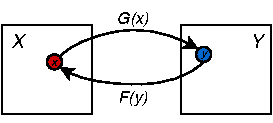
\includegraphics[width=0.4\textwidth]{img/cyc}
				\caption{Схема круговой согласованности для двух доменов \(X\) и \(Y\)}{
					\(x\) -- изображение домена \(X\), \(y\) -- изображение домена \(Y\)
				}
				\label{pic:cyc}
			\end{figure}
			\noindent
			Математически, можно сформулировать цикловую согласованность для случая двух доменов, формально введенного выше, в виде задачи минимизации следующей функции:
			\begin{equation}\label{eq:cc}
				\mathcal{L}_{\text{\tiny CC}}(G,F) = \mathbb{E}_{x}\big[\| F(G(x))-x \|\big] + \mathbb{E}_{y}\big[\| G(F(y))-y \|\big]
			\end{equation}
			Данный способ и его модификации используют многие методы в задачах обучения без учителя.
			Определенных успехов добились в этих работах~\cite{UNIT,MUNIT,CycleGAN}.
			Рассмотрим наиболее известные алгоритмы последних лет, в которых решаются задачи переноса изображения без учителя и которые можно применить к задаче дня и ночи.

		\paragraph{Состязательные сети с цикловой согласованностью}

			Исследовательская группа при университете Беркли, предложившая метод переноса с учителем pix2pix~\cite{pix2pix} (глава~\ref{sec:pix2pix}),
			признала, что для многих задач переноса изображений парное обучение будет неприменимым.
			Авторы представили новый метод, основанный на генеративно-состязательных сетях с цикловой согласованностью и на обучении без учителя~\cite{CycleGAN}, написанный на языке Lua с использованием Torch.
			Новый метод, получивший название CycleGAN, быстро обрел свою популярность, появилось множество его модификаций и реализаций в том числе и с использованием PyTorch.
			\newline
			\newline
			В основу метода лег все тот же pix2pix с его условными состязательными сетями, см. подробнее в главе~\ref{sec:pix2pix}, с тем отличием, что теперь тренировочная выборка была без заранее сформированных пар.
			Также в работе используется круговая согласованность генеративной сети, то есть модель обучается, не только переносить объекты между доменами, но и восстанавливать исходные изображения обратным переносом.
			
			\begin{figure}[ht]
				\centering
				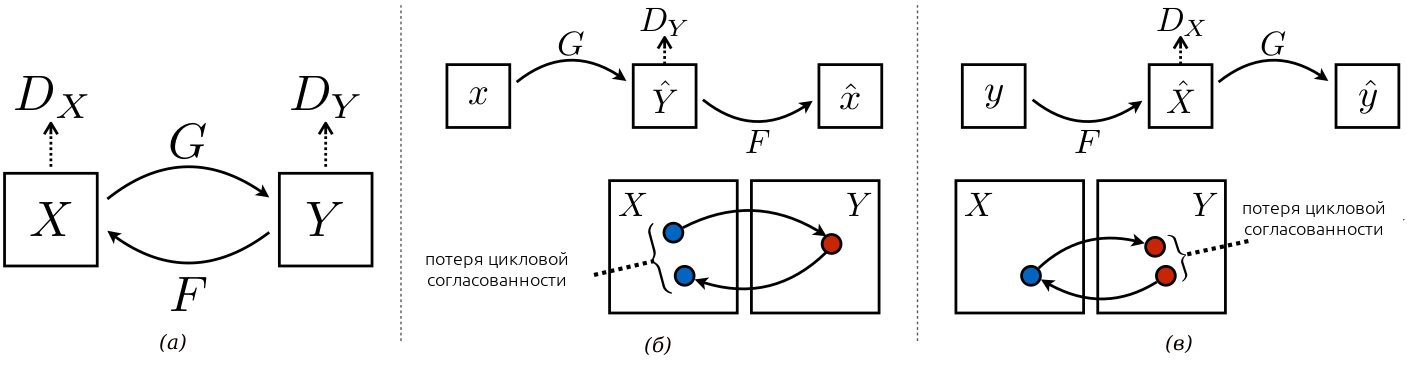
\includegraphics[width=0.9\textwidth]{img/cyclegan}
				\caption{Схема цикловой согласованностьи состязательных сетей CycleGAN}{
					\small{
						(а) модель состоит из двух отображений \(G: X \rightarrow Y\) и \(F: Y \rightarrow X\), и двух состязательных дискриминаторов \(D_Y\) и \(D_X\),
						для регулирования переноса используются (б) прямая цикловая согласованность: \(x \rightarrow G(x) \rightarrow F(G(x)) \approx x \),
						и (в) обратная: \(y \rightarrow F(y) \rightarrow G(F(y)) \approx y \)
					}}
				\label{pic:cyclegan}
			\end{figure}

			\noindent 
			В модели используются две состязательные сети:
			\begin{itemize}
				\setlength\parskip{0pt}
				\vspace{-0.5em}
				\item дискриминатор \(D_X\), отличающий изображения \(\{x\}, x \in X\) от перенесенных \(\{F(y)\}\)
				\item дискриминатор \(D_Y\), отличающий изображения \(\{y\}, y \in Y\) от перенесенных \(\{G(x)\}\)
			\end{itemize}
			\(D_X\) заставляет генератор \(G\) переносить изображения из \(X\) в изображения неотличимые от домена \(Y\), аналогично \(D_Y\) поощряет \(F\) синтезировать изображения близкие к \(X\).
			Авторы ввели функции потерь цикловой согласованности \(\mathcal{L}_{\text{\tiny CC}}\)~\eqref{eq:cc} и две функции состязательных потерь \(\mathcal{L}_{\text{\tiny GAN}_{\text{\tiny X}}}\) и \(\mathcal{L}_{\text{\tiny GAN}_{\text{\tiny Y}}}\)~\eqref{eq:gan}.
			Получилась следующая задача оптимизации:

			\begin{equation}\label{eq:cyclegan}
				\arg\min_{G, F}\max_{D_X, D_Y}\mathcal{L}_{\text{\tiny GAN}_{\text{\tiny X}}}(D_X,F,Y,X) + \mathcal{L}_{\text{\tiny GAN}_{\text{\tiny Y}}}(D_Y,G,X,Y) + \lambda\mathcal{L}_{\text{\tiny CC}}(G,F)
			\end{equation}
			Круговая согласованность генеративных сетей модели схематически изображена на рис.~\ref{pic:cyclegan}.

			\begin{figure}[ht]
				\centering
				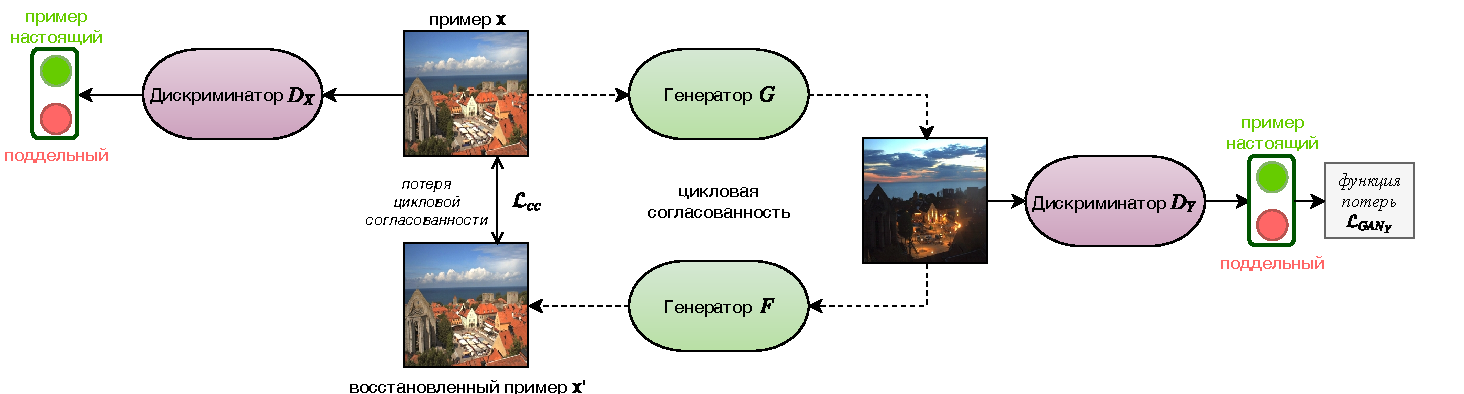
\includegraphics[width=0.9\textwidth]{img/cyclegan_model}
				\caption[Схема верхнеуровневой архитектуры CycleGAN (день в ночь)]{Схема верхнеуровневой архитектуры CycleGAN (день в ночь)\footnotemark}
				\label{pic:cyclegan_model}
			\end{figure}  \footnotetext{ для случая ночь в день, необходимо сменить местами генераторы и дискримианаторы, и по аналогии}
			\noindent
			Выше, на рис.~\ref{pic:cyclegan_model}, представлена верхнеуровневая логика реализуемой системы без учителя для случая изменения времени суток со дня на ночь. 
			
			\textbf{Архитектура CycleGAN} представляет собой глубокую сверточную нейронную сеть, основанную на остаточной сети ResNet~\cite{resnet}.
			Сеть поддерживает два режима обучения в зависимости от разрешения изображений обучающей выборки.
			В случае 128x128px и ниже используется 6 остаточных блоков ResNet, а в случаях 256x256px и выше их количество увеличивается до 9.
			Архитектуру генератора можно разбить на три части: сверточную, трансформирующую и декодирующую.
			Сверточная часть состоит из трех сверточных слоев, уменьшающих исходное изображение в 4 раза,
			трансформирующая часть содержит 6 или 9 остаточных блоков, в зависимости от параметров сети, требующаяся для объединения и наложения признаков изображения,
			последняя часть состоит из двух обратных сверточных слоев, необходимы для возвращения матрицы изображения к исходной размерности, и одного выходного слоя, преобразующего матрицу в RGB изображение.
			
			\begin{figure}[ht]
				\centering
				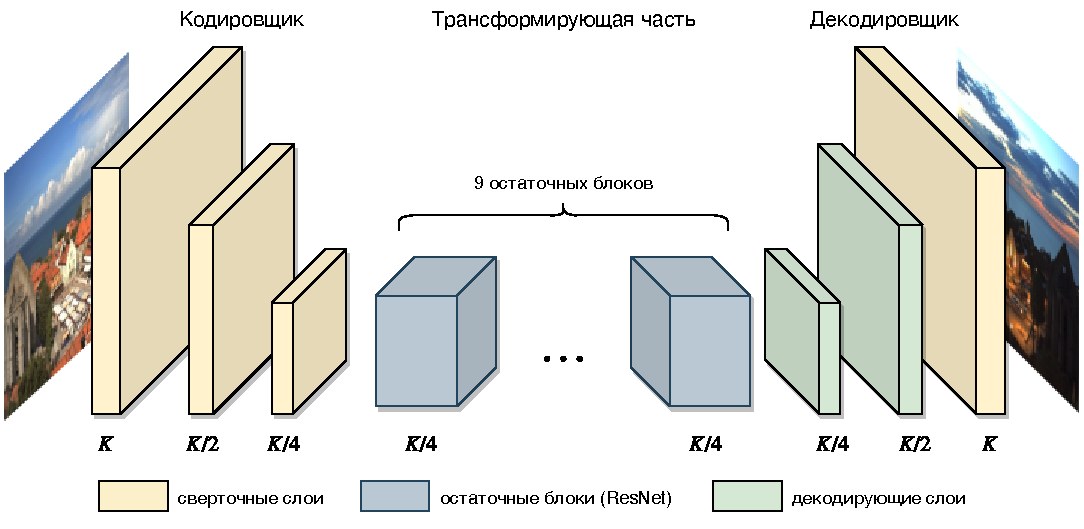
\includegraphics[width=0.9\textwidth]{img/cyclegan_gen}
				\caption{Архитектура генератора CycleGAN}{
					\small{
						Каждый слой завершается instance-нормализацией и слоем ReLU.\\
						$K$ -- исходный размер изображения

					}
				}
				\label{pic:cyclegan_gen}
			\end{figure}
			\noindent
			Благодаря сверточной структуре генератора, применить обученную сеть можно к изображению любого разрешения.
			На рис.~\ref{pic:cyclegan_gen} представлена схема сверточной сети генератора.
			В качестве архитектурного решения для дискриминатора был выбран тот же PatchGAN (см. подробнее на рис.~\ref{pic:cyclegan_dis}), уже показавший неплохие результаты в pix2pix~\cite{pix2pix}.
			PatchGAN -- это дискриминатор генеративно-состязательной сети, получающий на вход наложенные друг на друга части исходного изображения, ''патчи''.
			Результатом работы такого дискриминатора является матрица вероятностей, каждый элемент которой хранит вероятность того, что соответствующий ''патч'' настоящий.
			
			\begin{figure}[ht]
				\centering
				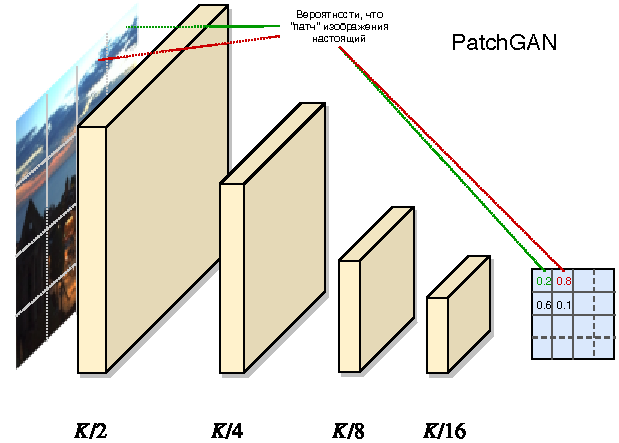
\includegraphics[width=0.54\textwidth]{img/cyclegan_dis}
				\caption{Архитектура дискриминатора PatchGAN}{
					\small{
						(каждый слой завершается instance-нормализацией и слоем ReLU)\\
						На вход подается разбитое изображение в масштабе 70x70px -- на выходе имеем матрицу вероятостей, что каждая отдельная часть является настоящей
					}
				}
				\label{pic:cyclegan_dis}
			\end{figure}

			\noindent
			Результаты работы CycleGAN превосходят по качеству все методы обучения без учителя, выходившие до этого
			и почти достигают по точности методы парного обучения.
			На сегодняшний день, эта работа показывает один из самых достойных результатов переноса изображений без учителя.
			При всех достоинствах алгоритма, задачи требующие существенных геометрических изменений на изображениях, например перенос кошки в собаку, зачастую терпят неудачу и требуют внесения ряда изменений~\cite{CycleGAN}.
			\newline\newline
			У сети появилось и продолжает появляться множество конкурентов~\cite{BicycleGAN,MUNIT,UNIT,DRIT}.
			Одним из первых успешных алгоритмов без учителя и прямым конкурентом CycleGAN, можно считать вот эту работу исследователей из NVIDIA~\cite{UNIT}.
			Модель, получившая название UNIT\footnote{
				\textbf{UNIT} (расш. англ. \textit{UNsupervised Image-to-Image Translationns})
			}, основана на архитектуре схожей с~\cite{CycleGAN}, но выполняет ряд дополнительных предположений о распределении данных, а также включает в себя
			вариационные автоэнкодеры, глава~\ref{sec:vae}, что позволяет разрешить проблемы искажений при геометрических преобразованиях у CycleGAN.
		
		\subsubsection*{Взаимосвязные состязательные сети (coGAN)}\label{sec:cogan}

			Взаимосвязные генеративно состязательные сети представляют собой надстройку над обычными состязательными сетями~\cite{coGAN}.
			CoGAN состоят из объединения двух сетей GAN, каждая сеть относится к своему домену.
			Взаимосвязные сети позволяют решать задачи поиска совместного распределения на непарных данных,
			что позволяет производить обучение на наборах данных без какой-либо заранее сформированной связи между объектами.
			Основной идеей coGAN является связь первых слоев генераторов \(G_1\) и \(G_2\), отвечающими за декодирование верхеуровневой семантики, и обмен весами между ними,
			аналогично связаны последние слои у дискриминаторов \(D_1\) и \(D_2\), отвечающие за кодирование верхнеуровневой семантики. 
			На данном подходе основываются генеративные сети в UNIT~\cite{UNIT}. 

		\subsubsection{Состязательные сети с общим скрытым пространством}\label{sec:latent}

			Создатели UNIT в своей работе используют связку VAE-GAN, что позволяет добиться реалистичности при непарном переносе изображений.
			Состязательные сети в моделе основаны на взаимосвязанных GAN (coGAN), с обменом параметрами весов между первыми слоями генераторов \(G_1\) и \(G_2\), см. главу~\ref{sec:cogan}.
			По этой же логике связаны последние высокоуровневые слои кодировщиков \(E_1\) и \(E_2\). 
			
			Авторы вводят понятие общего скрытого пространства \(\mathcal{Z}\), как гипотетического пространства скрытых переменных {\(\{z\}\), являющегося общим для каждого из доменов изображений.
			Формализовать эту теорию можно математически. Пусть у двух доменов изображений \(X_1\) и \(X_2\), между которыми планируется перенос, задано общее скрытое пространство \(\mathcal{Z}\).
			Пусть для каждого \(x_1 \in X_1, x_2 \in X_2\) существует общий латентный код \(z\) в пространстве \(\mathcal{Z}\).
			Тогда существуют такие функции, что выполняются следующие соотношения:
			
			\begin{equation}
				\begin{aligned}
					E_1(x_1) = &E_2(x_2) = z\\
					G_1(z) &= x_1\\
					G_2(z) &= x_2
				\end{aligned}
			\end{equation}
			А весь процесс переноса изображений между доменами \(X_1\) и \(X_2\), можно представить в виде композиции функции \(F_{1 \rightarrow 2}(x_1) = G_2(E_1(x_1)) = x_2\),
			и обратно \(F_{2 \rightarrow 1}(x_2) = G_1(E_2(x_2)) = x_1\). 

			\begin{figure}[ht]
				\centering
				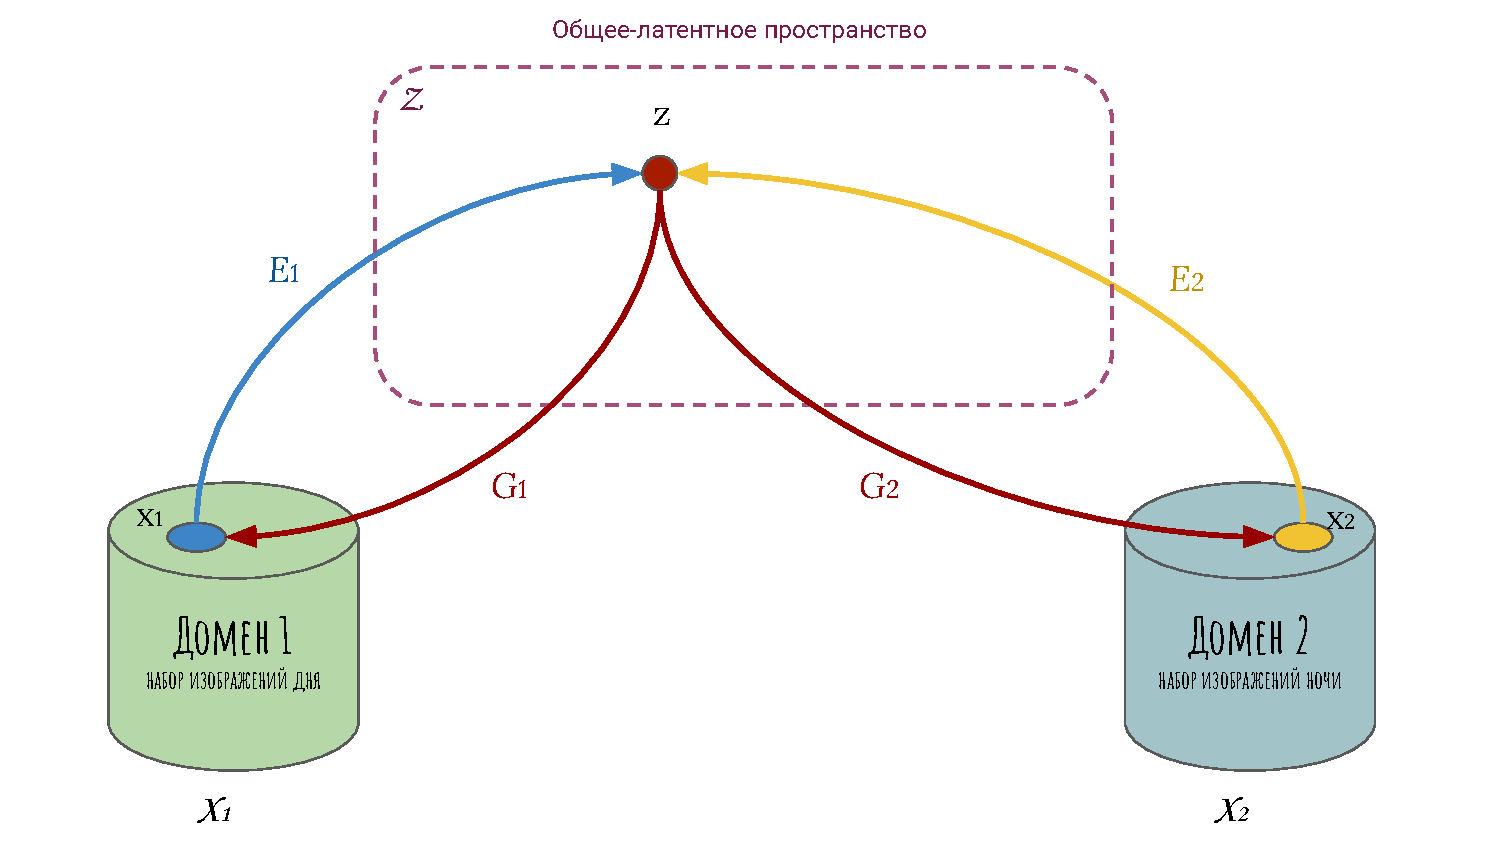
\includegraphics[width=0.8\textwidth]{img/unit}
				\caption{Схема работы VAE-GAN состязательных сетей с общим скрытым пространством}{
					\small{
						\(z\) -- код в скрытом пространсве \(Z\), \(x_1\) -- пример дня из домена \(X_1\),
						\(x_2\) -- пример ночи из домена \(X_2\), \(E_1\) -- энкодер сети для домена \(X_1\),
						\(E_2\) -- энкодер сети для домена \(X_2\), \(G_1\) -- генератор, синтезирующий изображения дня из скрытого представления,
						\(G_2\) -- генератор, создающий изображения ночи из скрытого представления.
					}
				}
				\label{pic:unit}
			\end{figure}
			\noindent
			Схематически работа связанных VAE-GAN состязательных сетей с общим латентным пространством для двух доменов изображена на рис.~\ref{pic:unit}.
			
			\noindent
			Можно заметить, что предположение об общем скрытом пространсве одновременно подразумевает цикловую согласованность, глава~\ref{sec:cc}. 


	\subsection{Выводы}

		Подводя итог, после рассмотрения различных методов по переносу изображений, стало ясно, что для задачи изменения времени суток на изображении подойдут
		алгоритмы обучения без учителя, поскольку обучение по парам, хоть и дает хорошие результаты, но из-за сложностей в сборе тренировочных данных, проигрывает непарным методам по числу задач, в которых оно применимо.
		Обучение без учителя же позволяет с легкостью собирать данные и находить зависимости между доменами, после чего синтезировать изображения на основе этой зависимости.
		Поэтому область применения таких методов намного шире, чем в моделях с учителем. 
		
		После исследования алгоритмов, я определил, что наиболее удачными являются методы основанные на GAN с круговой согласованностью~\cite[CycleGAN]{CycleGAN} и~\cite[UNIT]{UNIT}.
		Они используют схожие архитектуры и получают близкие результаты~\cite{UNIT_vs_CycleGAN},
		но UNIT обладает более сложной структурой из 6 связанных сверточных нейросетей: вариационных автокодировщиков и взаимосвязных состязательных сетей,
		что в перспективе дает более гибкую настройку и пространсво для маневров и расширений, поэтому в моей работе основной моделью выступает именно UNIT, но также проводится обучение и сравнение с CycleGAN. 
		
		Исходя из изучения методов без учителя, для реализации поставленой задачи потребуются собрать значительную базу изображений разичных времен суток.
		Авторы просмотренных мной работ не предоставляют доступы к внутренним датасетам лабораторий для обучения, поэтому под сбор данных я отвел отдельную подзадачу и подробнее о ее результатах расскажу в разделе~\ref{sec:data}.


\newpage
\section{Архитектура нейронной сети}\label{sec:model}

		В качестве архитектурного решения в работе используется сверточная нейронная сеть, состоящая из двух взаимосвязных генеративно состязательных сетей (coGAN, глава~\ref{sec:cogan}) и двух связных вариационных автоэнкодеров (VAE, глава~\ref{sec:vae}).
		Данный подход был предложен в статье~\cite{UNIT} и основан на предположении об общем скрытом пространстве переменных двух доменов, которое было описано в разделе~\ref{sec:latent}.
		
		\subsection{Домены изображений}\label{sec:model:domains}
			
			Модель подразумевает обучение без учителя на непарных данных, то есть на наборах классифицированных изображениях, не имеющих заранее установленных связей и меток.
			В архитектуре заложено использование двух доменов, поэтому для решения задачи необходимо заранее распределить тренировочные данные между ними.
			Подробнее сбор и классификация данных будут описаны в разделе~\ref{sec:data}. Сейчас остановимся на архитектурном решении загрузки и манипуляции изображениями в сети.

			Для двух различных доменов \(X_1\) и \(X_2\) настроены загрузчики данных, выполняющие загрузку, преобразование и отправку изображений в модель.
			Для аугментации данных\footnote{
				\textbf{Аугментация данных} (англ. \textit{augmentation}) -- увеличение общего числа данных, посредством преобразований над исходными данными 
			}
			в загрузчкике используются композиция трех видов преобразований входных изображений:

			\begin{enumerate}
				\item Изменение размера (resize) -- уменьшение или увеличение разрешения изображения
				\item Обрезка (crop) -- обрезание входного изображения в произвольном месте
				\item Отражение (flip) -- отражение входящих изображений по вертикали
			\end{enumerate}
			\noindent
			Далее преобразованные данные считывают кодировщики \(E_1\) и \(E_2\).

		\subsection{Вариационные автокодировщики}\label{sec:model:vae}

			В сети используются вариационные автокодировщики (VAE), их описание уже было проведено в разделе~\ref{sec:vae}. В ахитектуре модели используется два таких автокодировщика для каждого из доменов.
			VAE состоят из связанных кодировщиков \(E_1\) и \(E_2\), и двух связных генераторов \(G_1\) и \(G_2\).
			Первому домену соответствует автокодировщик \(\{ E_1,G_1 \}\), второму -- \(\{ E_2,G_2 \}\).
			Каждый энкодер получает на вход очередное изображения своего домена, сворачивает его в общий скрытый код \(z\).
			Последние высокоуровневые слои \(E_1\) и \(E_2\) связаны и обмениваются параметрами весов, что дает прирост в точности~\cite{coGAN}.
			Декодеры, они же генераторы, переносят изображение между доменами \(X_1\) и \(X_2\)~\eqref{eq:unit_translation} и восстанавливают исходное изображение из скрытого представления~\eqref{eq:unit_reconstruction}:
			\begin{equation}\label{eq:unit_translation}
				\begin{aligned}
					G_1(z_2 \sim q_2(z_2|x_2)) &= \tilde{x}^{2 \rightarrow 1}_2 \\
					G_2(z_1 \sim q_1(z_1|x_1)) &= \tilde{x}^{1 \rightarrow 2}_1 
				\end{aligned}
			\end{equation}
			\begin{equation}\label{eq:unit_reconstruction}
				\begin{aligned}
					G_1(z_1 \sim q_1(z_1|x_1)) &= \tilde{x}^{1 \rightarrow 1}_1 \\
					G_2(z_2 \sim q_2(z_2|x_2)) &= \tilde{x}^{2 \rightarrow 2}_2
				\end{aligned}
			\end{equation}

			\noindent
			Здесь \(z_1 \sim q_1(z_1|x_1)\) произвольное возмущенние от скрытого представления \(z\) с распределением Гаусса и единичной дисперсией \(q_1(z_1|x_1) \equiv \mathcal{N}(z_1|E_1(x_1), I)\),
			аналогично \(z_2\) получается из \(z\) с распределением \(q_2(z_2|x_2) \equiv \mathcal{N}(z_2|E_2(x_2), I)\).

			\begin{figure}[ht]
				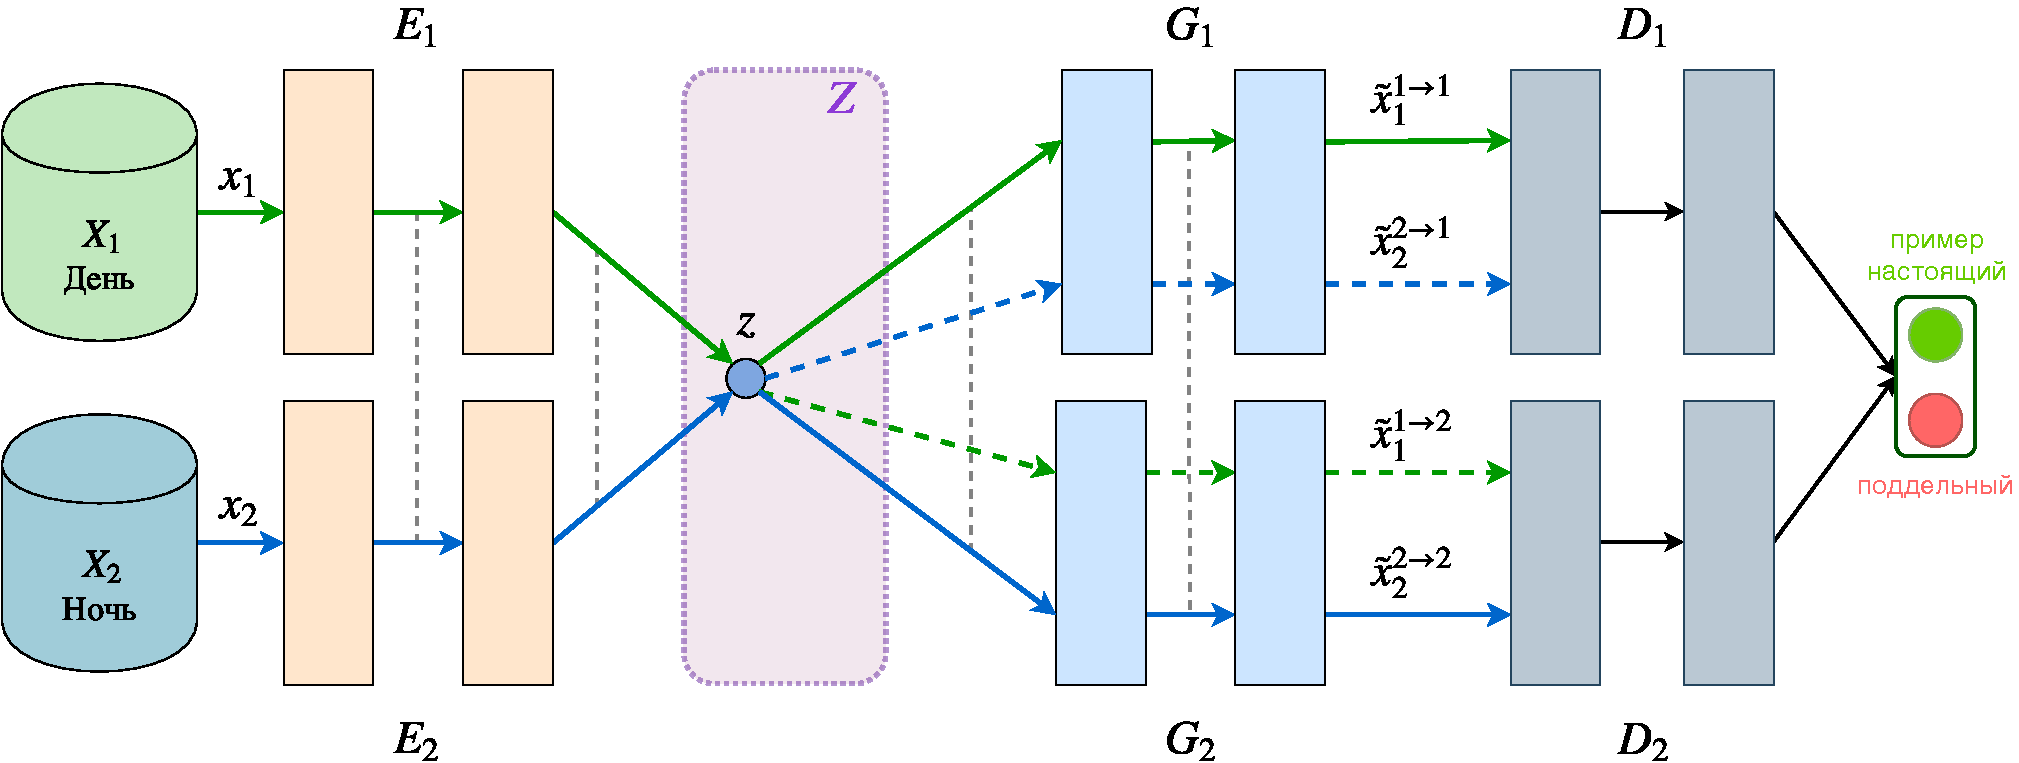
\includegraphics[width=1\textwidth]{img/unit_model}
					\caption{Схема используемой в работе сверточной нейронной сети}{
						\small{
							Кодировщики \(E_1,E_2\) преобразуют изображения в скрытый представление \(z\),
							генераторы \(G_1,G_2\) восстанавливают изображения \(\tilde{x}^{1 \rightarrow 1}_1,\tilde{x}^{2 \rightarrow 2}_2\) (сплошные стрелки)
							и переносят изображения в противоположные домены \(\tilde{x}^{1 \rightarrow 2}_1, \tilde{x}^{2 \rightarrow 1}_2\) из скрытого представления (пунктирные стрелки),
							дискриминаторы \(D_1,D_2\) отвечают за реалистичность и отличают настоящие изображения \((x_1, x_2)\) от сгенерированных \((\tilde{x}_2^{2 \rightarrow 1},\tilde{x}_1^{1 \rightarrow 2})\).
							Поскольку восстановление изображений контролируется сетью, GAN достаточно применять к перенесенным изображениям. 
							Пунктирными серыми линиями отражены связи между последними слоями кодировщиков и первыми слоями генераторов, отвечающими за извлечение верхнеуровневой информации.
						}}
				\label{pic:model}
			\end{figure}

			\noindent
			Полная схема работы нейронной сети, используемой в работе, представлена на рис.~\ref{pic:model}.
			Целью обучения VAE является минимизация следующих функций потерь~\eqref{eq:unit_vae}: 
			\begin{equation}\label{eq:unit_vae}
				\begin{aligned}
					\mathcal{L}_{\text{\tiny VAE}_1}(E_1,G_1)=&\lambda_1 \mathbb{KL}\big( q_1(z_1|x_1) \| p_{\eta}(z) \big) - \lambda_2 \mathbb{E}_{z_1 \sim q_1 (z_1|x_1)}\big[\log p_{G_1}(x_1|z_1)\big]\\
					\mathcal{L}_{\text{\tiny VAE}_2}(E_2,G_2)=&\lambda_1 \mathbb{KL}\big( q_2(z_2|x_2) \| p_{\eta}(z) \big) - \lambda_2 \mathbb{E}_{z_2 \sim q_2 (z_2|x_2)}\big[\log p_{G_2}(x_2|z_2)\big], \text{ где }
				\end{aligned}
			\end{equation}
			параметры \(\lambda_1\) и \(\lambda_2\) контролируют вклад соответствующих членов.
			
		\subsection{Генеративно состязательные сети}\label{sec:model:gan}

			Помимо вариационных автоэнкодеров в модели используются связанная пара генеративно-состязательных сетей GAN.
			Первый GAN состоит из генератора \(G_1\) и дискриминатора \(D_1\), вторая состязательная сеть -- из \(G_2\) и \(D_2\). 
			Генераторы уже были описаны в предыдущем подпункте.
			Дискриминаторы на вход получают настоящее изображение из соответствующего домена и перенесенное генератором из другого, и возвращают вероятности того, что изображения настоящие.
			\newline\newline
			Функции потерь состязательных сетей можно записать в виде:
			\begin{equation}\label{eq:unit_gan}
				\begin{aligned}
					\mathcal{L}_{\text{\tiny GAN}_1}&(E_2,G_1,D_1)=\lambda_0\mathbb{E}_{x_1 \sim P_{\mathcal{X}_1}} \big[\log D_1 (x_1) ]+\lambda_0\mathbb{E}_{z_2 \sim q_2 (z_2|x_2)}\big[\log(1-D_1(G_1(z_2)))\big]\\
					\mathcal{L}_{\text{\tiny GAN}_2}&(E_1,G_2,D_2)=\lambda_0\mathbb{E}_{x_2 \sim P_{\mathcal{X}_2}} \big[\log D_2 (x_2) ]+\lambda_0\mathbb{E}_{z_1 \sim q_1 (z_1|x_1)}\big[\log(1-D_2(G_2(z_1)))\big], \text{ где }
				\end{aligned}
			\end{equation}
			гиперпараметр \(\lambda_0\) отвечает за вклад соответствующих членов.
			\newpage\noindent
			Таким образом, архитектура сети состоит из двух кодировщиков, двух генераторов и двух состязательных дискриминаторов. 
			Модель решает сразу несколько подзадач и обучает одновременно несколько подсетей.
			Ключевой целью является оптимизация минимаксной задачи:

			\begin{equation}\label{eq:unit_loss}
				\begin{aligned}
					\min_{E_1,E_2,G_1,G_2} \max_{D_1,D_2} 
					&\mathcal{L}_{\text{\tiny VAE}_1}(E_1,G_1) +\mathcal{L}_{\text{\tiny GAN}_1}(E_2,G_1,D_1) +\mathcal{L}_{\text{\tiny CC}_1}(E_1,G_1,E_2,G_2)\ +\\
					&\mathcal{L}_{\text{\tiny VAE}_2}(E_2,G_2) + \mathcal{L}_{\text{\tiny GAN}_2}(E_1,G_2,D_2)+\mathcal{L}_{\text{\tiny CC}_2}(E_2,G_2,E_1,G_1), \text{ где }
				\end{aligned}
			\end{equation}
			функции потерь \(\mathcal{L}_{\text{\tiny VAE}} =\)~\eqref{eq:unit_vae} и \(\mathcal{L}_{\text{\tiny GAN}} = \)~\eqref{eq:unit_gan}, а потеря круговой согласованности \(\mathcal{L_{\text{\tiny CC}}}\) получается из функции:
			\begin{equation}\label{eq:unit_cc}
				\begin{aligned}
					\mathcal{L}_{\text{\tiny CC}_1}(E_1,G_1,E_2,G_2)=&\lambda_3\mathbb{KL}\big( q_1(z_1|x_1) \| p_{\eta}(z) \big)+\lambda_3\mathbb{KL}\big( q_2(z_2|x_1^{1\rightarrow 2}) \| p_{\eta}(z) \big)\ -\\
					&\lambda_4\mathbb{E}_{z_2 \sim q_2 (z_2|x_1^{1 \rightarrow 2})}\big[\log p_{G_1}(x_1|z_2)\big]\\
					\mathcal{L}_{\text{\tiny CC}_2}(E_2,G_2,E_1,G_1)=&\lambda_3\mathbb{KL}\big( q_2(z_2|x_2) \| p_{\eta}(z) \big)+\lambda_3\mathbb{KL}\big( q_1(z_1|x_2^{2\rightarrow 1}) \| p_{\eta}(z) \big)\ -\\
					&\lambda_4\mathbb{E}_{z_1 \sim q_1 (z_1|x_2^{2 \rightarrow 1})}\big[\log p_{G_2}(x_2|z_1)\big].
				\end{aligned}
			\end{equation}
			гиперпараметры \(\lambda_3\) и \(\lambda_4\) управляют вкладом соответствующих компонент.

			\begin{table}[h]
				\centering
				\begin{tabular}{|
					>{\columncolor[HTML]{B7CCC3}}c|c|c|c|c|c|}
					\hline
					\textbf{Сети} & ${E_1,G_1}$   & ${E_1,G_2}$                   & ${G_1,D_1}$   & ${E_1,G_1,D_1}$ & ${G_1,G_2,D_1,D_2}$ \\ \hline
					\textbf{Роли} & VAE для $X_1$ & Перенос $X_1 \rightarrow X_2$ & GAN для $X_1$ & VAE-GAN         & CoGAN~\cite{coGAN}  \\ \hline
				\end{tabular}
				\caption{Роли подсетей в используемой модели}
				\label{tab:nets}
			\end{table}
			\noindent
			В таблице~\ref{tab:nets} представлены роли подсетей используемой модели.

		\subsection{Сверточная сеть выделения признаков}\label{sec:model:vgg}
			 
			Для выделения признаков на изображениях, в моей работе используется глубокая сверточная сеть VGG16~\cite{vgg}, рис.~\ref{pic:vgg16}.

			\begin{figure}[ht]
				\centering
				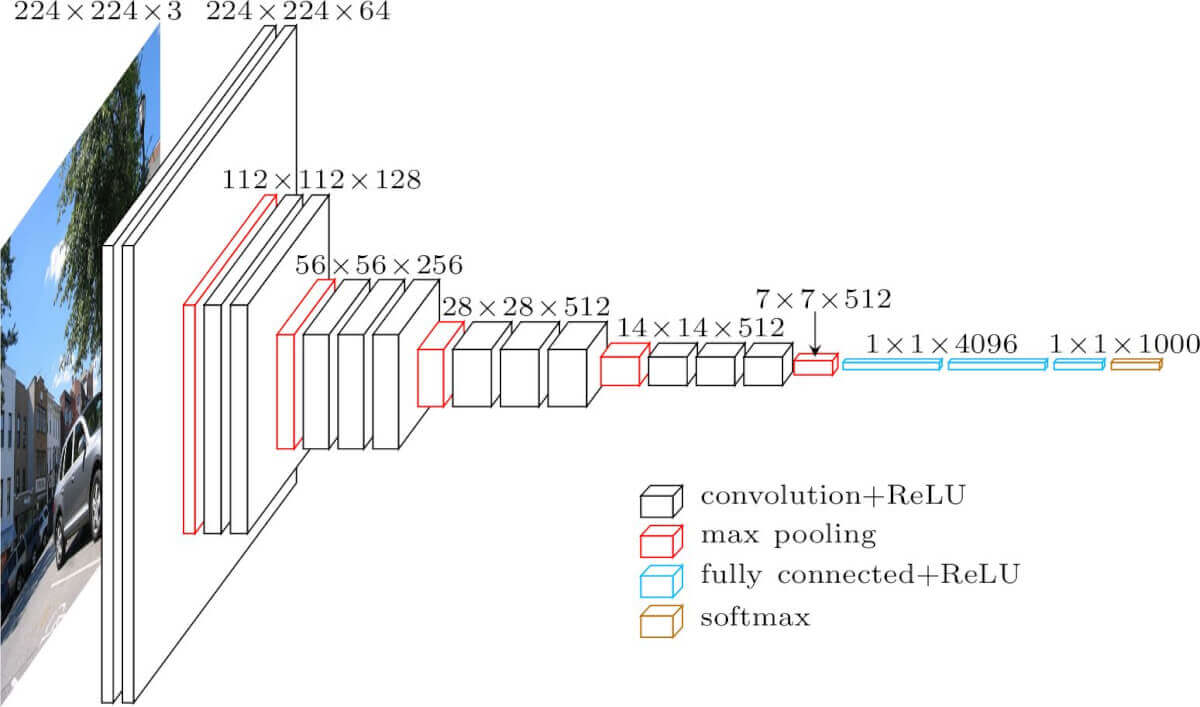
\includegraphics[width=0.85\textwidth]{img/vgg16}
				\caption{Модель глубокой сверточной сети VGG16}
				\label{pic:vgg16}
			\end{figure}
			
			\noindent 
			VGG16 -- это сеть нового поколения, построенная как усовершенствованная версия AlexNet~\cite{AlexNet}. 
			VGG сопоставимая по точности с ResNet, но в обучении без учителя обладает большей стабильностью~\cite{MUNIT}.
			В процессе экспериментов проводится оценка качества работы модели как с использованием сверточной сети VGG16, так и без нее.

		\subsection{Нормализация}\label{sec:model:norm}

			В процессе обучения были использованы различные стратегии повышения качества выходных изображений.
			Одним из подходов было применения слоев нормализации в генеративно-состязательных сетях.
			Всего было реализованы три типа нормализации: батч-нормализация~\cite{n_batch}, слой-нормализация~\cite{n_layer} и instance-нормализация~\cite{n_instance}.

			\noindent
			Общий вид вычисления нормализации можно записать следующим образом:
			\begin{equation}\label{eq:norm}
				\hat{x} = \frac{x - mean(\bar{x})}{std(\bar{x})}, \text{ где }
			\end{equation}
			mean -- среднее значение, std -- дисперсия. 
			
			Использование нормализаций позволяет существенно ускорить обучение нейронной сети.
			Одним из самых популярных видов нормировки является батч-нормализация, представленная в 2015 году в этой работе~\cite{n_batch}.
			Авторы предлагают считать среднее значение от суммы всех тензоров в батче, после чего подсчитывать дисперсию и для каждого примера вычислять~\eqref{eq:norm}.
			Чем больше размер батча, тем эффективнее будет работа нормализации.

			Другой подход применяют в этой работе~\cite{n_layer}, где предлагают вычислять слой-нормализацию вдоль входа, что дает независимое значение для каждого примера и позволяет использовать ее в модели даже при единичном размере батча.
			
			Авторы instance-нормализации~\cite{n_instance}, продолжают идею слой-нормализаций, и вычисление происходит по каждому каналу каждого входного примера.
			Идеи каждой из нормализаций изображены на мнемонической схеме~\ref{pic:norm}.

			\begin{figure}[ht]
				\centering
				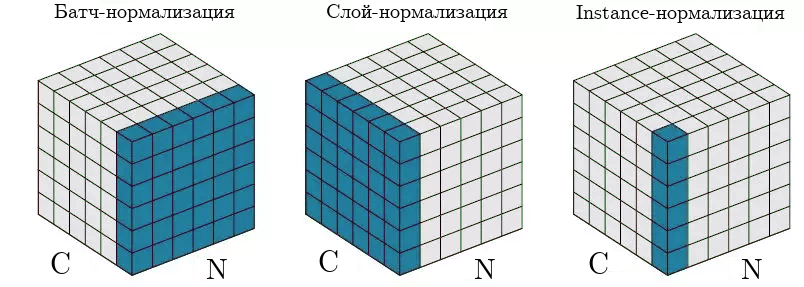
\includegraphics[width=0.9\textwidth]{img/norm}
				\caption{Виды нормализации используемые в обучении}{
					\small{
						C -- число каналов, N -- размер батча
					}
				}
				\label{pic:norm}
			\end{figure}

\newpage
\section{Проведенное исследование}
	
	\subsection{Собранная база изображений}\label{sec:data}
		
		Обучение без учителя глубоких сверточных сетей требуют большого объема тренировочных данных.
		Количество изображений, для получения достойных результатов, может варьироваться от нескольких сотен до десятков тысяч и больше.
		Во многих разобранных мной статьях, авторы, помимо описания алгоритма и демонстрации результатов, дают возможность провести самостоятельное обучение на предложенных датасетах или воспользоваться предобученными моделями.
		К сожалению, авторами не было предоставлено публичных наборов данных или предобученных моделей на тему изменения времени суток.
		Поэтому в своем исследовании, я выделил сбор требуемых данных и оценку их репрезентативности в отдельную подзадачу.
		
		\subsubsection*{Возникшие трудности}\label{sec:difficulties}
		После исследования области, оказалось, что основная проблема, заключается не в поиске данных, а в их разметке. Многие датасеты поставляются или с бесполезной для решения моей задачи разметкой, или в принципе без нее.
		Из всех найденных мной датасетов, которые теоретически возможно применить к поставленной задаче, самыми крупными и в наилучшем качестве, были наборы фотографий с автомобильных видеорегистраторов.
		Наиболее подходящие датасеты, которые я обнаружил: 
		
		\begin{enumerate}
			\item NEXET~\cite{data:nexet} -- набор из 50тыс. разнообразных дорожных размеченных изображений дня, ночи и сумерек. Данные расположены в одной директории, метки хранятся в \texttt{.csv} файле.
			\item BDD100K~\cite{data:bdd100k} -- набор из 100тыс. разнообразных дорожных изображений, изображения разбиты на тестовую и тренировочную выборки в соотношении 2:7, размечены только тренировочные данные, метки хранятся в \texttt{.json} файле.
			\item Alderley DayNight~\cite{data:alderley} -- набор из 15тыс. пар дорожных изображений, предоставлены в виде двух доменов: дня и ночи. 
			\item Night2Day Paired~\cite{data:paired_night2day} -- набор из 17тыс. пар изображений c веб-камер в низком разрешении, предоставлены соединенными.
		\end{enumerate}
		\noindent
		Из датасетов выше:~\cite{data:alderley,data:paired_night2day} содержат недостаточное число изображений в низком разрешении для непарного переноса обучения. Alderley представляет собой кадры снятые только в одном месте -- в пригороде Олдерли, Квинсленд.
		Night2Day содержат всего 101 уникальную пару и применяются в этой работе обучения с учителем~\cite{pix2pix}, рис.~\ref{pic:pix2pix_results}.
		Такие данные больше подходят для парного обучения с учителем, в своей же работе я использую методы без учителя, поэтому мой выбор пал на два наиболее качественных датасета: NEXET и BDD100K.
		Датасеты содержат большое число изображений в высоком разрешении 720p с различной погодой и отснятых в разных городах, и отлично подходят для обучения выбранной нейронной сети.
		
		\subsubsection*{Классификация изображений}\label{sec:classify_images}

			Набор данных NEXET поставляется с файлом меток \text{train.csv} с тремя типами меток (день, ночь, сумерки), но как оказалось многие из них не соответствуют действительности, см.~рис~\ref{pic:nexet_mis}.
			
			\noindent
			Изображения размечались в рамках соревнования~\cite{data:nexet}, поэтому в наборе присутствуют спорные данные, неприминимые в обучении, так например целая метка ''Сумерки'' не представляет ценности, так как на ней могут быть как и яркие изображения, так и темные.
			Также никак не выделяются фотографии снятые в подземных парковках, туннелях и гаражах.
			Датасет BDD100K имеет более гибкие метки: ночь, день, рассвет/сумерки и неопределенность, в местах где нет однозначного ответа.

			\begin{figure}[ht]
				\centering
				\begin{subfigure}[ht]{0.49\textwidth}
					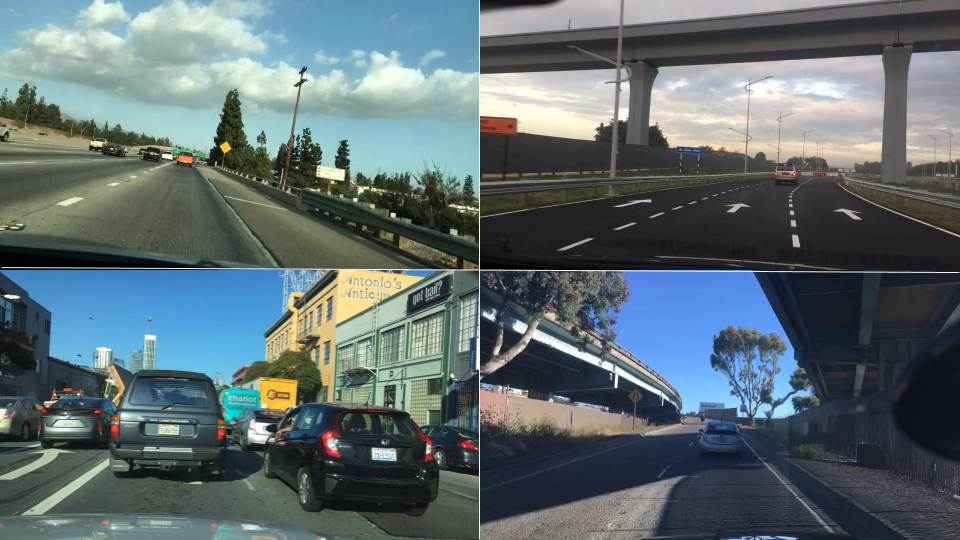
\includegraphics[width=\textwidth]{img/nexet_mis_night}
					\caption{метки ночи}
				\end{subfigure}
				\begin{subfigure}[ht]{0.49\textwidth}
					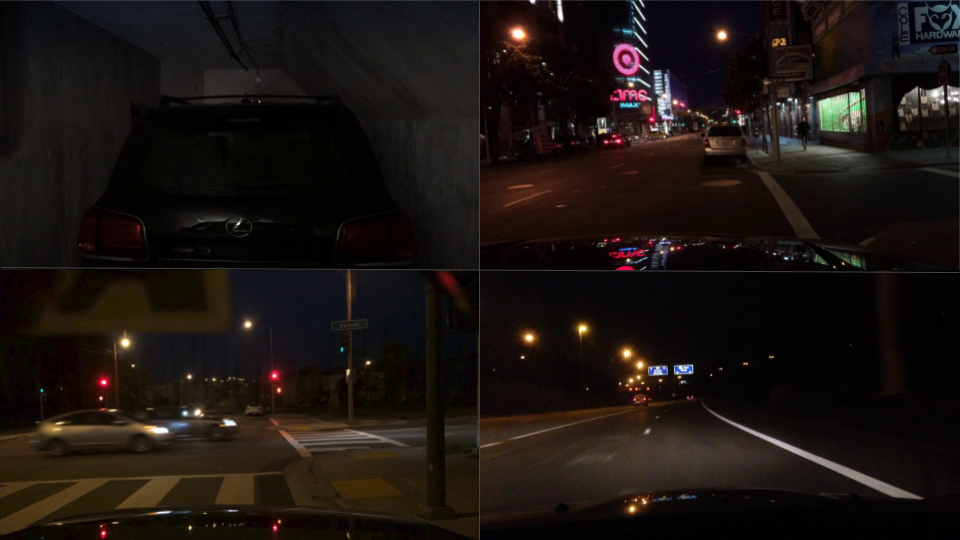
\includegraphics[width=\textwidth]{img/nexet_mis_day}
					\caption{метки дня}
				\end{subfigure}
				\caption{Пример ошибочного сопоставления меток NEXET}{
					\small{
					(a) -- примеры изображения с выставленными метками ночи,
					(b) -- примеры изображения с выставленными метками дня, помимо явно ошибочных изображений, также присутствуют спорные (верхнее левое, (b)), например, изображения на подземных парковках и туннелях
				}}
				\label{pic:nexet_mis}
			\end{figure}

			\noindent
			Для исправляющей разметки датасетов был написан Python скрипт \texttt{detect\_day\_night.py}, определяющий время суток по яркости изображения.
			Результат применения его к одному из датасетов ниже:
			\begin{figure}[ht]
				\centering
				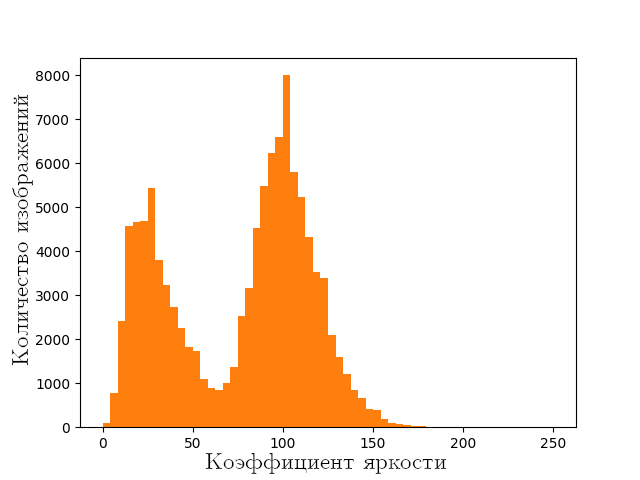
\includegraphics[width=0.6\textwidth]{img/histogram60}
				\caption{Гистограмма распределения яркости изображений в датасете NEXET}{
					\small{
						возвышение слева -- коэфициент яркости меньше, темнее, ночь;
						возвышение справа -- день
					}
				}
				\label{pic:hist_detect}
			\end{figure}

			\noindent
			Эксперементальным путем было установлено, что данные находящиеся по коэффициенту яркости в дипозоне от \(60 < \gamma \le 68\) с большей вероятностью относятся к спорным данным.
			Скрипт проводит сравнение с официальной разметкой, где выявляет несовпадения, после чего явно ошибочные данные отделяются от тренировочных.
			
		

		\subsubsection*{Распределение собранных данных на домены}

			В своей работе я использовал несколько различных стратегий разбиения данных.
			Всего в сети используется 4 домена: два тренировочных и два тестовых.
			Обучение проходило на изображениях из датасета NEXET~\cite{data:nexet}, с распределением тренировочных и тестовых примеров в соотношених 9:1 и 1:1.
			Проводилась искуственная аугментация данных: отражения, обрезания и изменения размера, о чем уже упомяналось в разделе~\ref{sec:model:domains}.
			Помимо этого, обучение проходило и на размеченных данных, без отделения от ошибочных и на соовокупности с датасетом BDD100K~\cite{data:bdd100k}, затем выполнялось сравнение полученных результатов.
			
			
	\subsection{Эксперименты}\label{sec:tests}

		Обучение глубокой сверточной нейронной сети на базе изображений высокого разрешения требует внушительных вычислительных ресурсов.
		Так как тренировка проводилась на графических картах, основная нагрузка ложилась на ядра CUDA и видеопамять GPU.
		
		Одно полное обучение может занимать от двух до 12 дней, в зависимости от параметров сети.
		Свои эксперименты я в основном производил на видеокартах c 12GB видеопамяти.
		Для датасета с изображениями в разрешении 256х256 пикселей требовалось 4700MB видеопамяти, а для изображений 512х288 пикселей -- более 8.5GB.
		Ниже приведены график зависимости скорости обучения от используемой видеокарты, рис.~\ref{pic:gpu_power}, и таблица связи используемой памяти от разрешения изображений, табл.~\ref{tab:memory}.

		\begin{figure}[ht]
			\centering
			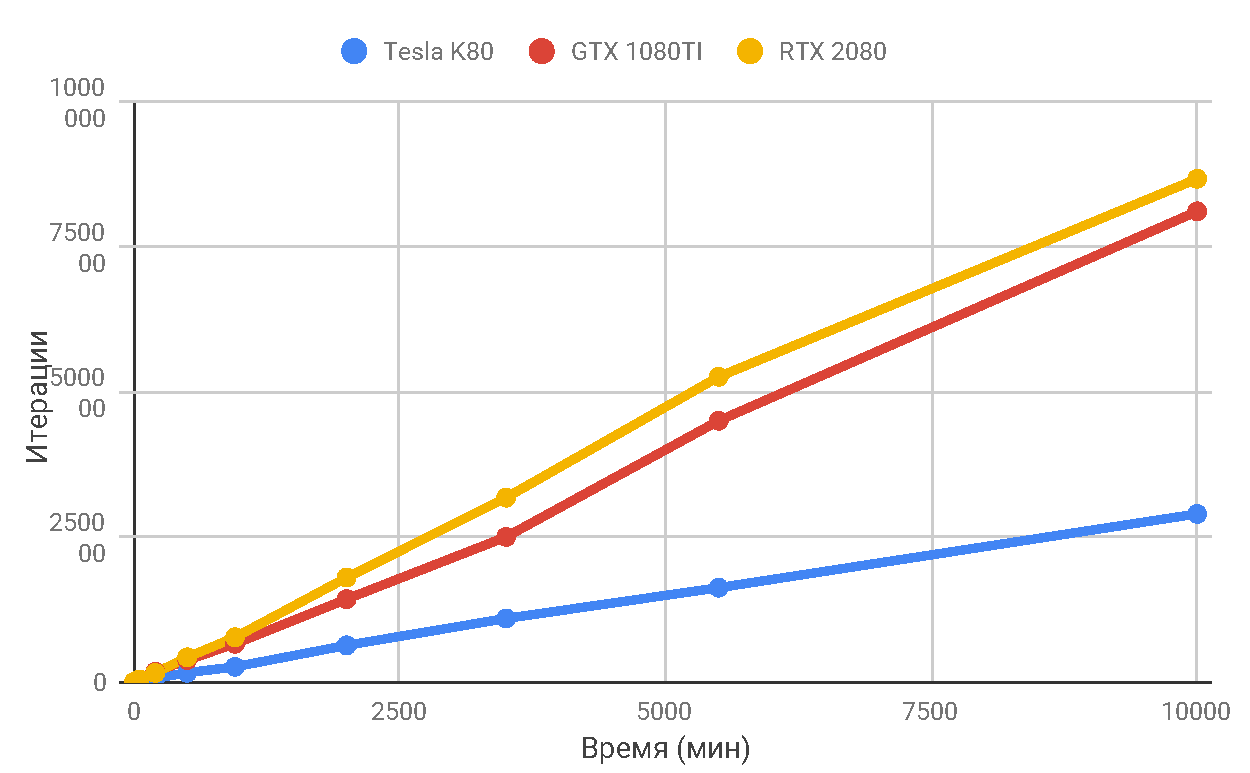
\includegraphics[width=0.7\textwidth]{img/gpu_power}
			\caption{Зависимость скорости обучения от GPU}
			\label{pic:gpu_power}
		\end{figure}

		\begin{table}[ht]
			\centering
			\begin{tabular}{|c|c|c|}
				\hline
				\rowcolor[HTML]{EFEFEF}
				\textbf{Разрешение изображений} & \textbf{Видеопамять, VRAM} & \textbf{С использованием VGG16} \\ \hline
				64х64 px                        & 1630 MB                         & 1720 MB                       \\ \hline
				128x128 px                      & 2014 MB                         & 2156 MB                       \\ \hline
				256x256 px                      & 4384 MB                         & 4752 MB                       \\ \hline
				512x288 px                      & 7678 MB                         & 8550 MB                       \\ \hline
			\end{tabular}
			\caption{Зависимость используемой памяти от разрешения и VGG16}
			\label{tab:memory}
		\end{table}			
		
		\noindent
		В процессе обучения использовалось до 7 графических карт (3 различных). 
		Самой быстрой себя показала графическая карта RTX 2080, близкие результаты у GTX 1080TI, поэтому основная часть обучения проводилась на них.
		Tesla K80 предоставляется на сервере Google Colab~\cite{colab}, и при большем количестве графических ядер CUDA, показывает худший результат.
		Скорее всего, это происходит из-за того, что мощность серверной карты урезается искусственно, так как она находится в распределенном доступе с другими пользователями.
		Из графика~\ref{pic:gpu_power} также следует, что скорость обучения сети не меняется на всем протяжении обучения. 

		\subsubsection*{Проведенные эксперименты}
			
			В общей сложности было проведено более 15 полноценных обучений с различными параметрами нейронной сети и на разнообразных наборах данных.
			Эксперименты можно разделить на 4 основные группы: 
			\begin{itemize}
				\item \hyperref[sec:tests:nexet]{Эксперименты на базе изображений NEXET}~\cite{data:nexet}
				\item \hyperref[sec:tests:nexet_ext]{Эксперименты на базе NEXET с аугментацией данных}\footnotemark[1] (расширенной)
				\item \hyperref[sec:tests:nexet_no_err]{Эксперименты на расширенной базе NEXET с отделением от ошибочных изображений}
				\item \hyperref[sec:tests:nexet_bdd]{Эксперименты на объединенной базе NEXET + BDD100K}~\cite{data:bdd100k}
			\end{itemize}
			\footnotetext[1]{\textbf{Аугментация} -- искусственное расширение датасета: отражения, обрезания, изменения размера, см. подробнее раздел~\ref{sec:model:domains}}

			\noindent
			Одним из наиболее значимых параметров, влияющих на результаты сети, является параметр слоя нормализации.
			В модели всего было реализовано 4 различных типа нормализации.
			В таблице~\ref{tab:configs} приведены различные конфигурации сети используемые при обучении.
			
			\begin{table}[h]
				% \centering
				\begin{tabular}{|c|c|c|c|c|c|c|}
					\hline
					\rowcolor[HTML]{AFD7AF} 
					\cellcolor[HTML]{EFEFEF}{\color[HTML]{CB0000} \textbf{Параметры обучения}} & \multicolumn{4}{c|}{\cellcolor[HTML]{AFD7AF}\textbf{Используемые нормализации}} & \multicolumn{2}{c|}{\cellcolor[HTML]{F7C7B1}\textbf{Модели}}     \\ \hline
					\rowcolor[HTML]{AFD7AF} 
					\cellcolor[HTML]{B6C0D0}\textbf{Датасет}                                   & \textbf{Нет}     & \textbf{Batch}~\cite{n_batch}    & \textbf{Layer}~\cite{n_layer}    & \textbf{Instance}~\cite{n_instance}    & \cellcolor[HTML]{F7C7B1}\textbf{Нет} & \cellcolor[HTML]{F7C7B1}\textbf{VGG16} \\ \hline
					\rowcolor[HTML]{EFEFEF} 
					NEXET                                                                      & $\checkmark$     & \textbf{---}      & \textbf{---}      & \textbf{---}         & $\checkmark$                         & \textbf{---}                           \\ \hline
					NEXET+аугментация                                                        & $\checkmark$     & \textbf{---}      & \textbf{---}      & \textbf{---}         & $\checkmark$                         & $\checkmark$                           \\ \hline
					\rowcolor[HTML]{EFEFEF} 
					NEXET+скрипт\footnotemark[2]                                                & $\checkmark$     & $\checkmark$      & $\checkmark$      & $\checkmark$         & $\checkmark$                         & $\checkmark$                           \\ \hline
					NEXET+BDD100K                                                              & $\checkmark$	     & \textbf{---}      & $\checkmark$        & $\checkmark$         & \textbf{---}                         & \cellcolor[HTML]{FFFFFF}$\checkmark$   \\ \hline
				\end{tabular}
				\caption{Параметры нейронной сети в ходе экспериментов}{
					\small{
					}
				}
				\label{tab:configs}
			\end{table}
			\footnotetext[2]{\textbf{detect\_day\_night.py} -- скрипт для определения времени суток и отделения спорных данных от тренировочных, см. разделы~\ref{sec:difficulties} и~\ref{sec:classify_images}}
			
			\subsubsection{Эксперименты на базе изображений NEXET}\label{sec:tests:nexet}
				Датасет NEXET~\cite{data:nexet} содержит 50 тыс. изображений с метками дня, ночи и сумерек.
				Изначально была произведена попытка обучить сеть с разделеним на тестовые и тренировочные домены в соотношении 1:1.
				Сумерки использовались вместе с доменом ночи, табл.~\ref{tab:tests:nexet}, эксп.~1.
				\begin{table}[ht]
					\centering
					\begin{tabular}{|c|c|c|c|c|}
					\hline
					\rowcolor[HTML]{EFEFEF} 
					\multicolumn{1}{|l|}{\cellcolor[HTML]{EFEFEF}} & \multicolumn{2}{c|}{\cellcolor[HTML]{EFEFEF}\textbf{Эксперимент 1}} & \multicolumn{2}{c|}{\cellcolor[HTML]{EFEFEF}\textbf{Эксперимент 2}} \\ \hline
					\rowcolor[HTML]{EFEFEF} 
					\textbf{Домены\textbackslash{}Время}           & \textbf{День}                & \textbf{Ночь+Сумерки}                & \textbf{День}                    & \textbf{Ночь}                    \\ \hline
					\cellcolor[HTML]{EFEFEF}\textbf{Test}          & 12451                        & 12548                                & 4981                             & 4654                             \\ \hline
					\cellcolor[HTML]{EFEFEF}\textbf{Train}         & 12452                        & 12549                                & 19922                            & 18578                            \\ \hline
					\end{tabular}
					\caption{Разбиение датасетов для обучения на NEXET}
					\label{tab:tests:nexet}
				\end{table}

				\noindent
				Полученные результаты были далеки от идеала: преобразование ночи в день не получилось в принципе, на дне в ночь было множество артефактов.
				Тогда была предпринята попытка увеличить тренировочную выборку за счет уменьшения тестовой, было выбрано соотношение 8 к 2. 
				Также из обучения были убраны изображения сумерек (1874 шт.), поскольку их, по факту, невозможно было отнести ни к одному домену, так как под этой меткой могли скрываться как и дневные, так и ночные изображения, табл.~\ref{tab:tests:nexet}, эксп. 2.  
				
				Перенос ночи в день все также не удался, день в ночь стал немного лучше, но артефакты все еще присутствовали.

			\subsubsection{Эксперименты на расширенной базе NEXET}\label{sec:tests:nexet_ext}
				
				Так как существует положительная зависимость между качеством обучения модели и количеством тренировочных данных, следующей предпринятой попыткой было искусственное расширение датасета, или аугментация.
				О способах аугментации, уже было сказано в разделе~\ref{sec:model:domains}.
				Тренировочные и тестовые данные брались в отношении 9:1, чтобы максимизировать выборку для обучения, оставив достаточное количество изображений для валидации и оценки.
				
				Качество результатов заметно выросло, артефакты почти исчезли, но присутствовала проблема в переносе цвета и выделения признаков у разных объектов.
				Так, например, деревья подсвечивались как фонари или дома, рис.~\ref{pic:nexet_ext}.

				\begin{figure}[ht]
					\centering
					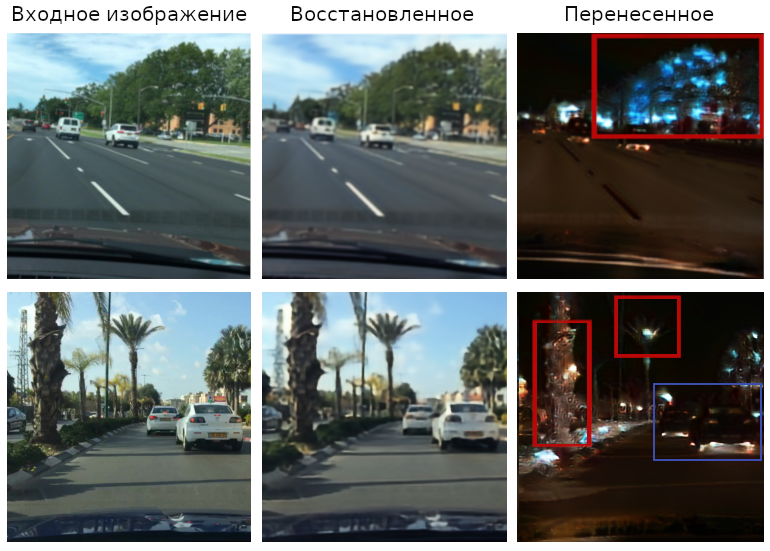
\includegraphics[width=0.8\textwidth]{img/nexet_ext}
					\caption{Пример ошибочного выделения признаков}{
						\small{
							{\color[HTML]{CB0000} \textbf{крассный --}} ошибка в выделении признаков, подсветка деревьев \\
							{\color[HTML]{3b4daf} \textbf{синий --}} ошибка в переносе цвета, затемнение машин
						}
					}
					\label{pic:nexet_ext}
				\end{figure}
				
				\noindent
				На этом этапе перенос ночи в день все еще был неуспешным. На перенесенных изображениях присутствовало большое число артефактов, а цвета были сильно искажены.
				Альтернативные стратегии разбиения данных на домены: другое соотношение тренировочных и тестовых примеров, изменение разрешения изображенй, перемешивание изображений -- также не увенчались успехом.
				

			\subsubsection{Эксперименты на расширенной базе без ошибочных изображений}\label{sec:tests:nexet_no_err}
				
				В процессе экспериментов у некоторых изображений были обнаружены несовпадения меток, рис.~\ref{pic:nexet_mis}. 
				Для решения проблемы с разметкой данных была написана программа помогающая классифицировать изображения, подробнее см. раздел~\ref{sec:classify_images}.

				После программной обработки датасета, оказалось, что более 5000 изображений имели несовпадающие метки.
				Отделив ошибочные данные и перегруппировав домены, обучение провелось еще раз.
				
				\begin{figure}[ht]
					\centering
					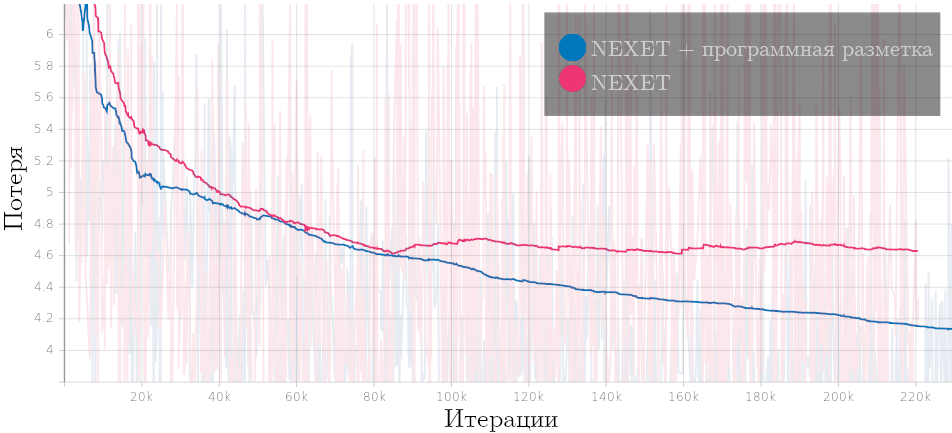
\includegraphics[width=0.9\textwidth]{img/loss_gen_no_err.png}
					\caption{Графики функция потерь NEXET после программной обработки}
					\label{pic:loss_gen_no_err}
				\end{figure}

				\noindent
				Как видно из графиков, на рис.~\ref{pic:loss_gen_no_err}, начиная с 85 тыс. итеарций потери модели на официальной разметке NEXET начинают колебаться около значения 4.7, когда как у датасета с программным удалением ошибочных данных обучение продожается, а функция потерь убывает. 
				На рисунке~\ref{pic:example_no_err} приведены примеры работы алгоритма.

				\begin{figure}[ht]
					\centering
					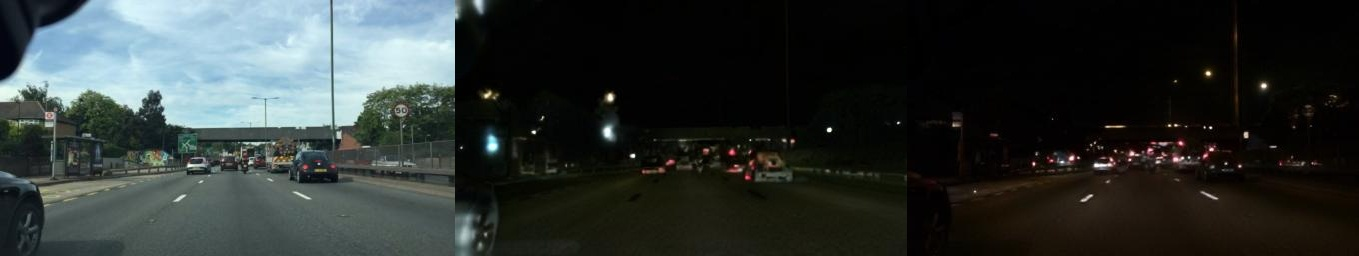
\includegraphics[width=0.9\textwidth]{img/example_no_err_2}
					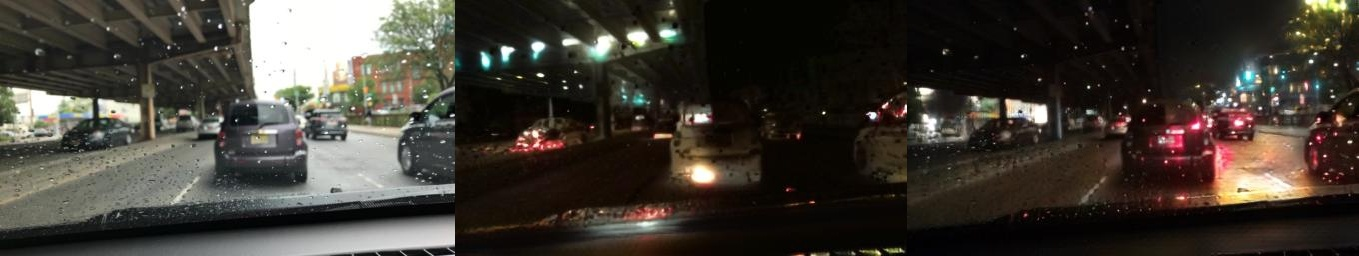
\includegraphics[width=0.9\textwidth]{img/example_no_err_1}
					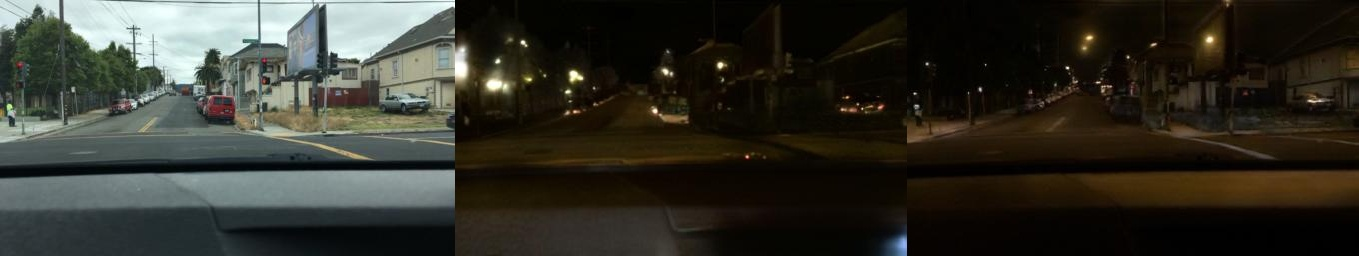
\includegraphics[width=0.9\textwidth]{img/example_no_err_3}
					\caption{Визуальное сравнение результатов модели с программной обработкой}{
						\small{
							слева-направо: вход, без обработки NEXET, с программной обработкой NEXET
						}
					}
					\label{pic:example_no_err}
				\end{figure}

				\newpage\noindent
				Дополнительно проводились эксперименты с добавлением слоев нормализации в GAN, см.~раздел~\ref{sec:model:norm}, что теоретически может разрешить проблему с искаженными цветами и засветами.
				Всего было использовано три различных подхода, табл.~\ref{tab:configs}.

				Батч-нормализация зависит от числа примеров одновременно участвующих в обучении~\cite{n_batch}. Это накладывает ограничение на размера батча снизу.
				После сравнения результатов работы модели с нормализацией и без нее -- визуальных улучшений обнаружено не было, поэтому дальнейшее обучение проводилось с размером минибатча равному одому, без батч-нормализации.

				Также использовались алтернативные стратегии: слой-нормализация (layer) и instance-нормализация, у которых нет зависимости от размера батча~\cite{n_layer,n_instance}, что дает им преимущество над нормализацией выше в случае единичного размера минибатча.
				
				Визуально результаты получались довольно близкие.
				Цвета передавались заметно точнее после применения к модели сверточной сети VGG16, подробнее в разделе~\ref{sec:model:vgg}.
				В соовокупности со слой-нормализацией удалось затемнить яркие контуры и минимизировать засветы.
				На рисунке~\ref{pic:vgg_no_vgg} представлен пример работы сети, с различными типами конфигураций.
				Пример выбран случайно из тестовой выборки.  

				
				\begin{figure}[ht]
					\centering
					\includegraphics[width=\textwidth]{img/vgg_norm_cmp}
					\caption{Сравнение результатов модели с нормализацией и VGG16}
					
					\label{pic:vgg_no_vgg}
				\end{figure}
				
			\subsubsection{Эксперименты на объединенной базе изображений NEXET и BDD100K}\label{sec:tests:nexet_bdd}
				
				Последняя группа экспериментов ставилась на наиболее крупной выборке, состоящей из двух датасетов: NEXET~\cite{data:nexet} и BDD100K~\cite{data:bdd100k}.
				Помимо всего прочего, к данным применялась аугментация и программное отделение ошибочных примеров, о которых уже было сказано в предыдущих разделах.
				Всего в обучении участвовало 140тыс. изображений.
				В общей сложности было поставлено 3 различных типа экспериментов с параметрами нормализации и VGG16 моделью, табл.~\ref{tab:configs}.
				\newline\newline
				На графике~\ref{pic:nexet_bdd} изображены функции потерь для генератора и дискриминатора на протяжении всего обучения.
				В начале обучения потери генераторов компенсировались потерями дискриминаторов, что затрудняло однозначно выделить победителя.
				Но в перспективе в районе 800 тыс. итераций, дискриминаторы показывали одинаковый результат, а генератор у BDD+NEXET показывал лучший.
				
				\begin{figure}[ht]
					\centering
					\begin{subfigure}[ht]{0.45\textwidth}
						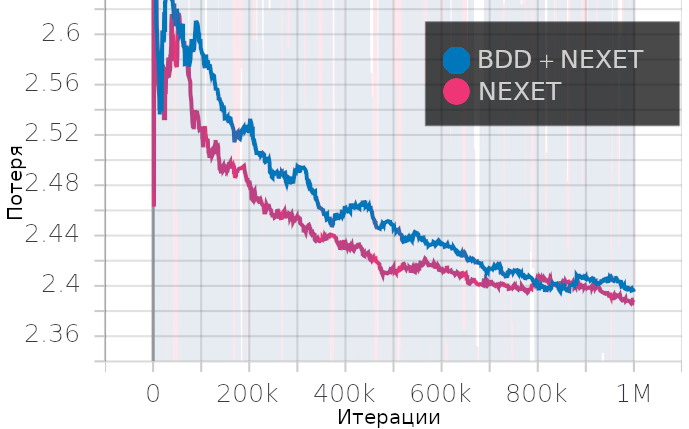
\includegraphics[width=\textwidth]{img/nexet_bdd_dis}
						\caption{Потеря дискриминатора}
					\end{subfigure}
					\begin{subfigure}[ht]{0.45\textwidth}
						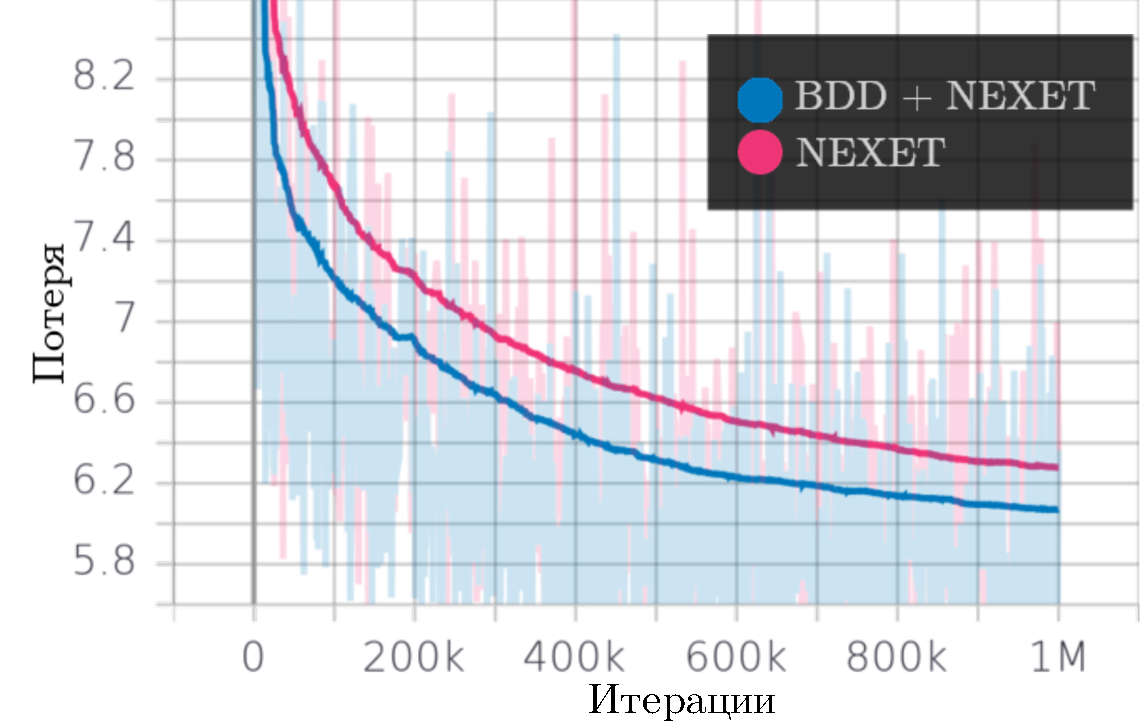
\includegraphics[width=\textwidth]{img/nexet_bdd_gen}
						\caption{Потеря генератора}
					\end{subfigure}
					\caption{Графики функция потерь при обучении на NEXET и на NEXET+BDD}
					\label{pic:nexet_bdd}
				\end{figure}

				\newpage\noindent
				После эксперементального сравнения с помощью метрики структурного сходства SSIM, было получено, что значение индекса в переносе из дня в ночь выше почти на 18\%, в переносе ночи в день -- на 7\%.
				Это дает основания полагать, что эксперемент на расширенной базе соовокупности двух датасетов можно считать успешным.
				
	\subsection{Эксперементальная оценка}\label{sec:eval}

		В обучении без учителя на непарных данных оценить качество модели являеется непростой задачей.
		Для оценки качества переноса были взяты две основные метрики SSIM (Structural Similarity,~\cite{metric:ssim}) и PSNR (Peak Signal-to-Noise Ratio).
		PSNR построена на вычислении среднего квадратического отклонения, и применить ее в обучении без учителя между противоположными доменами не представляется возможным, но при этом, она подходит для определения качества обучения по точности реконструкции модели.
		Метрика структурного сходства, напротив, позволяет сравнивать переносимое изображение с исходным, так как она учитывает структурное изменение информации.
		В табл.~\ref{tab:metrics} приведена эксперементальная оценка результатов работы программы.

		\begin{table}[ht]
			\centering
			\begin{tabular}{|c|c|c|c|c|c|c|}
				\hline
				\rowcolor[HTML]{EFEFEF} 
														& \multicolumn{2}{c|}{\cellcolor[HTML]{EFEFEF}\textbf{Перенос: A$\rightarrow$B}} & \multicolumn{2}{c|}{\cellcolor[HTML]{EFEFEF}\textbf{Перенос: B$\rightarrow$A}} & \multicolumn{2}{c|}{\cellcolor[HTML]{EFEFEF}\textbf{Реконструкция}} \\ \hline
				\rowcolor[HTML]{EFEFEF} 
				{\color[HTML]{9A0000} \textbf{Метрика}} & \textbf{CycleGAN}                       & \textbf{Модель}                      & \textbf{CycleGAN}                       & \textbf{Модель}                      & \textbf{CycleGAN}                 & \textbf{Модель}                 \\ \hline
				\cellcolor[HTML]{EFEFEF}\textbf{SSIM}   & 0.297                                   & 0.381                                & 0.390                                   & 0.405                                & 0.754                             & 0.954                           \\ \hline
				\cellcolor[HTML]{EFEFEF}\textbf{PSNR}   & -                                       & -                                    & -                                       & -                                    & 20.3                              & 33.7                            \\ \hline
				\end{tabular}
			\caption{Эксперементальная оценка работы модели}{
				\small{
					A -- домен дня, B -- домен ночи.
				}
			}
			\label{tab:metrics}
		\end{table}
		
		\subsubsection*{Оценка скорости работы предобученной модели}\label{sec:eval:speed}

			После продолжительного обучения результатом работы нейронной сети является предобученная модель, содержащая эмпирические параметры и веса сети, достачные для переноса изображений между доменами.
			Для итоговой модели была вычислена скорость работы, в зависимости от разрешения изображений и использования глубой сверточной сети VGG16.
			По результатам тестирования был построен график зависимости~\ref{pic:speedtest}.

			\begin{figure}[ht]
				\centering
				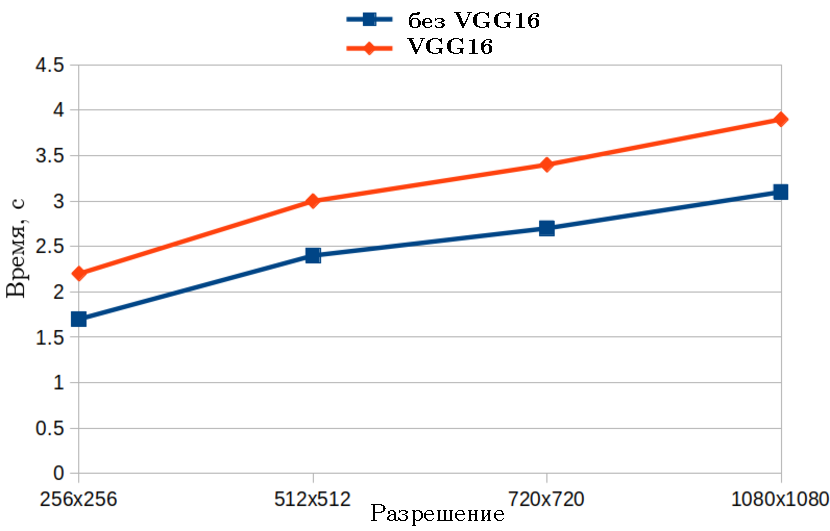
\includegraphics[width=0.75\textwidth]{img/speedtest}
				\caption{Зависимость времени работы модели от разрешения и VGG16}{
					(перенос между доменами одного изображения)
				}
				\label{pic:speedtest}
			\end{figure}
			

			
	\newpage
	\subsection{Результаты}\label{sec:results}

		\begin{figure}[ht]
			\centering
			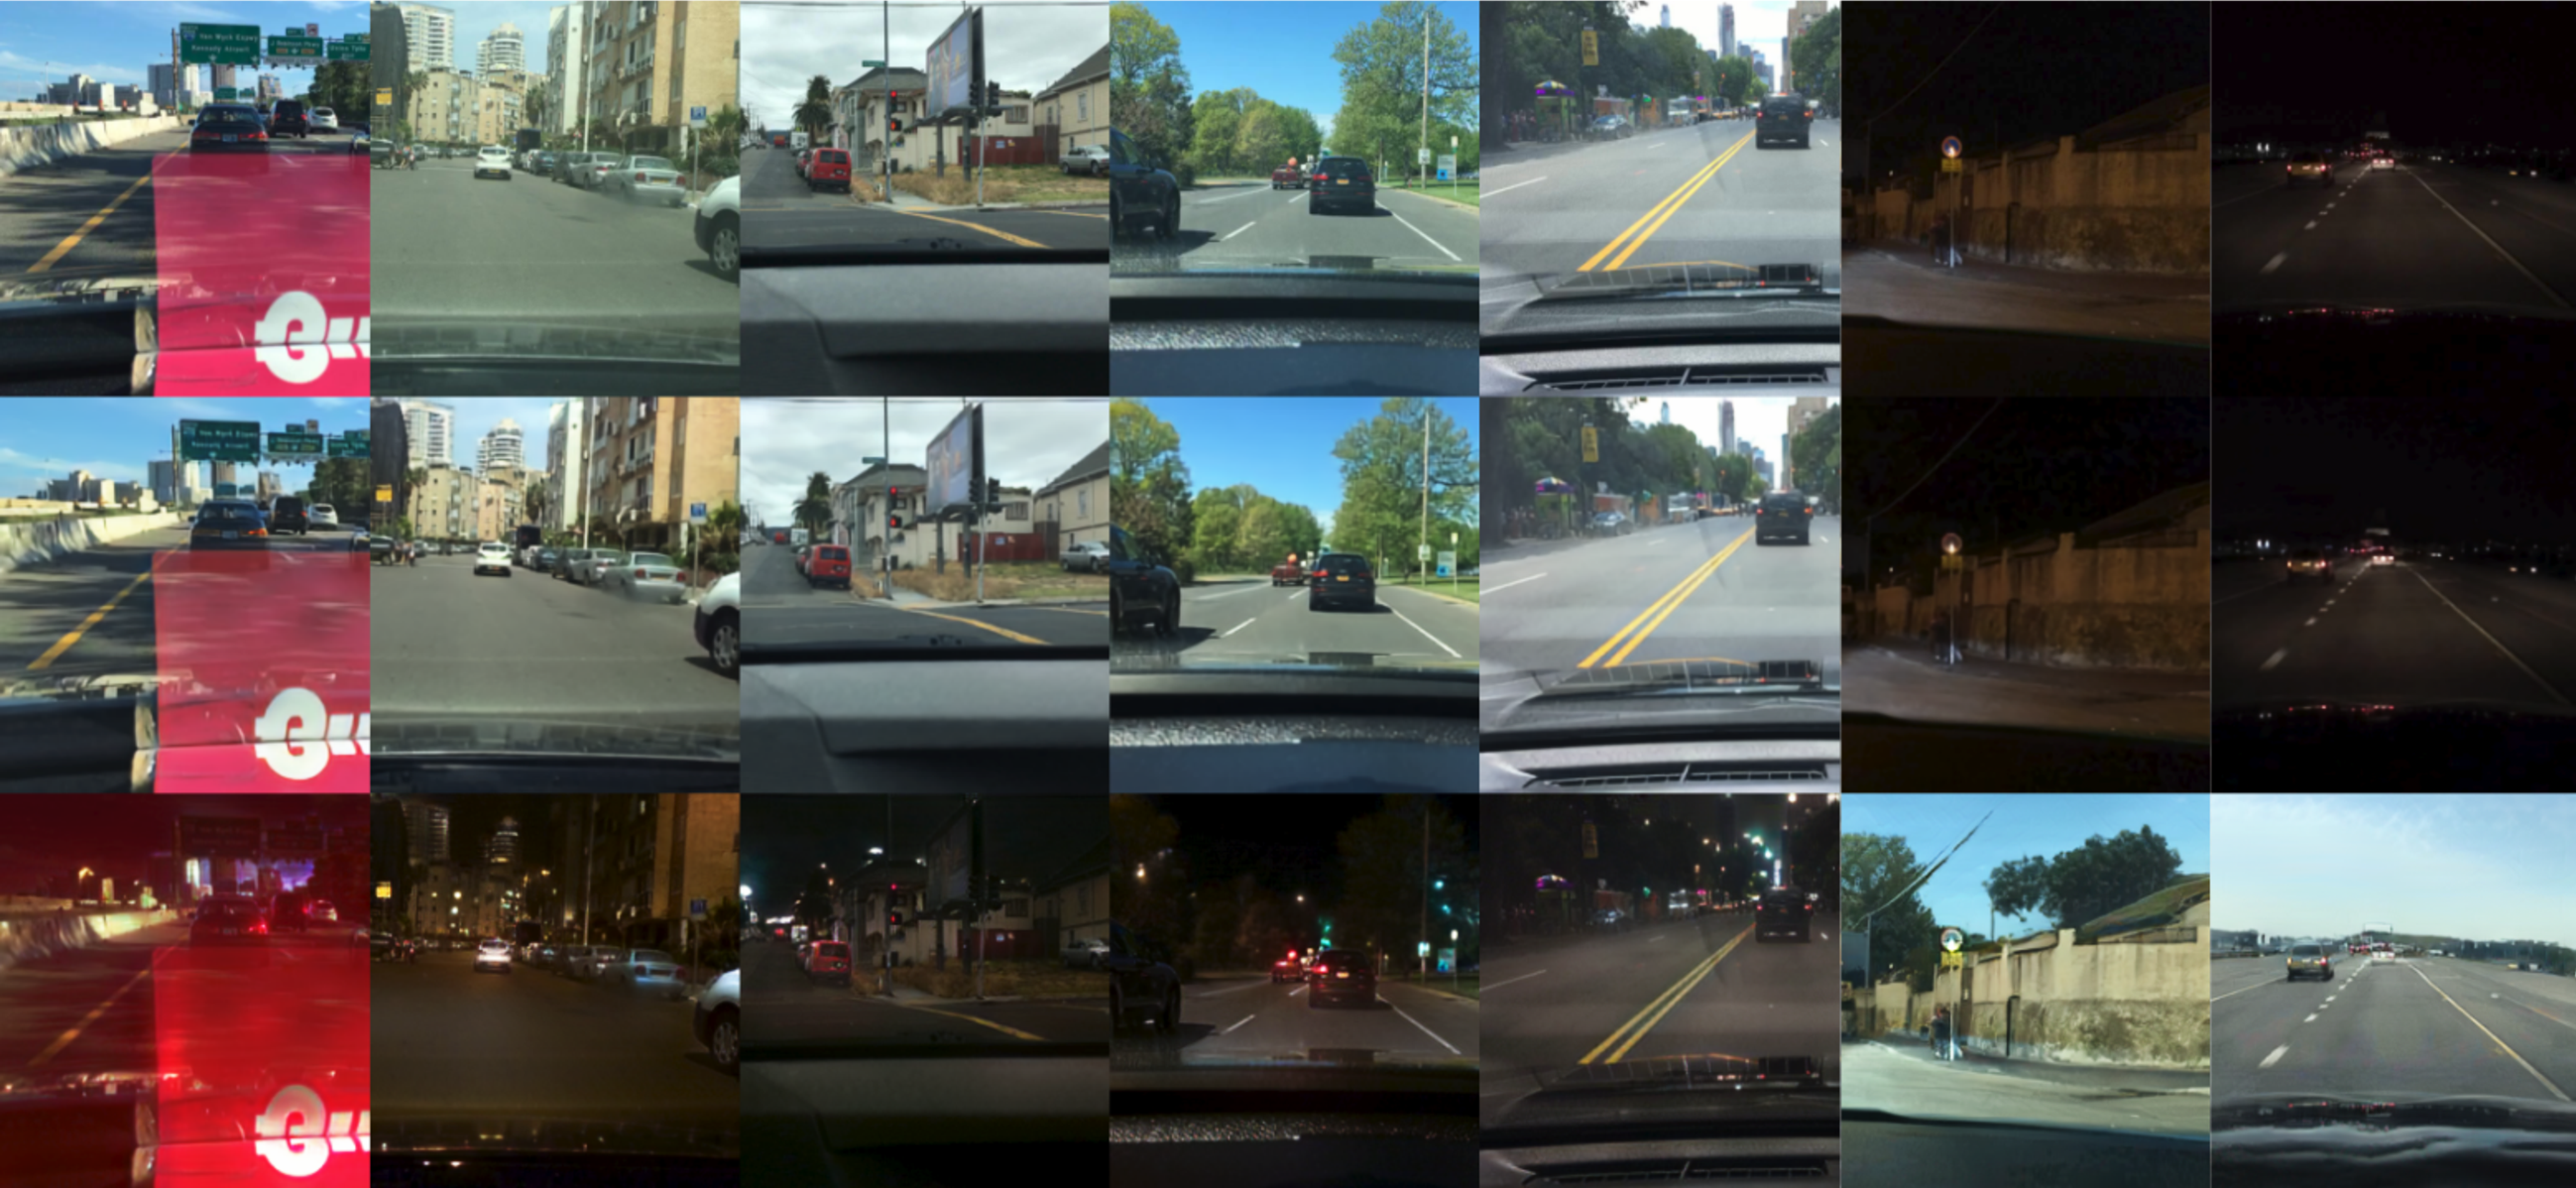
\includegraphics[width=\textwidth]{img/results}
			\caption{Результаты работы метода}{
				\small{
					сверху-вниз: вход, реконструкция, перенос между доменами
				}
			}
		\end{figure}

\newpage
\section{Программная реализация}\label{sec:prac}

	\subsection{Инструментарий}\label{sec:tools}

		В работе использованы различные средства для проведения вычислений и обучения.
		Большая часть экспериментов была поставлена на графических картах лаборатории: NVIDIA GTX 1080 Ti, но также вычисления проводились на сервере Google Colaboratory с помощью Tesla K80~\cite{colab} и на видеокарте NVIDIA RTX 2080.
		В качестве языка реализации был выбран Python 3.6.
		Все тесты проводились в виртуальных Docker контейнерах с предустановленной операционной системой семейства Linux, Ubuntu 18.04.
		Эксперементальная оценка была выполнена в интерактивной оболочке Jupyter Notebook, часть анализа работы алгоритма проводилась с помощью TensorBoard -- инструмента визуализации этапов обучения нейронных сетей.

	\subsection{Программный код}\label{sec:code}

		Всего было написано 7 программ на языке Python, выполняющие тестирование, подготовку данных для обучения и эксперементальную оценку результатов, общей сложностью более 800 строк кода.
		И более 250 строчек было написано для реализации обучения и модификации используемой нейронной сети. Репозиторий с исходный кодом~\cite{day2night}. 

		\subsubsection*{Библиотеки}
			Основными используемыми библиотеками были:
			
			\begin{compactlist}
				\item Pytorch -- весь каркас обучения, библиотека для работы с нейросетью
				\item OpenCV, Pillow, imageio -- библиотеки для работы с изображениями
				\item Pandas, Numpy -- для работы с большими объемами данных и вычислениями
				\item Matplotlib, Scikit-image -- библиотеки для экспериментальной оценки результатов
			\end{compactlist}
			
\newpage
\section{Заключение}\label{sec:conclusion}
	В рамках работы были решены следующие задачи:
	
	\begin{itemize}
		\item Проведен обзор существующих методов переноса изображений и анализ решений родственных задач
		\item Найдены применимых к проблеме тренировочные датасеты -- изображений с различными временем суток~\cite{data:nexet,data:bdd100k}
		\item Провелась классификация тренировочных данных и распределение данных по доменам 
		\item На основе проведенного исследования и обзора литературы, выбрана модель, подходящая для решения поставленной задачи
		наилучшим образом
		\item Проведена серия экспериментов переноса изображений, получена эксперементальная оценка качества и скорости работы модели 
	\end{itemize}



\newpage
\begin{thebibliography}{00}

	
	\bibitem{i2ipapers}
	\textbf{Supervised and Unsupervised Image Translation} --
	\href{https://github.com/lzhbrian/image-to-image-papers}{A collection of image to image papers with code},
	2019.

	\bibitem{style_transfer}
	\textbf{J.Johnson, A.Alahi, L.Fei-Fei}.
	\emph{Perceptual Losses for Real-Time Style Transfer and Super-Resolution}.
	Department of Computer Science, Stanford University,
	March 2016.

	\bibitem{color_transfer}
	\textbf{R.Zhang, J.-Y.Zhu, P.Isola, X.Geng, A.S.Lin, T.Yu, A.A.Efros}.
	\emph{Real-Time User-Guided Image Colorization with Learned Deep Priors}.
	University of California, Berkeley,
	May 2017.

	\bibitem{CycleGAN}
	\textbf{J.-Y.Zhu, T.Park, P.Isola, A.A.Efros}.
	\emph{Unpaired Image-to-Image Translation using Cycle-Consistent Adversarial Networks}.
	Berkeley AI Research (BAIR) laboratory, UC Berkeley,
	March 2017.

	\bibitem{pix2pix}
	\textbf{P.Isola, J.-Y.Zhu, T.Zhou, A.A.Efros}.
	\emph{Image-to-image translation with conditional adversarial networks}.
	Berkeley AI Research (BAIR) laboratory, UC Berkeley,
	November 2016.

	\bibitem{super_resolution}
	\textbf{Y.Yuan, S.Liu, J.Zhang, Y.Zhang, C.Dong, L.Lin}
	\emph{Unsupervised Image Super-Resolution using Cycle-in-Cycle Generative Adversarial Networks}
	Guangdong Key Laboratory of Intelligent Information Processing, Shenzhen University,
	Graduate School at Shenzhen, Department of Automation, Tsinghua University,
	September 2018.

	\bibitem{UNIT}
	\textbf{M.-Y.Liu, T.Breuel, J.Kautz}.
	\emph{Unsupervised Image-to-Image Translation Networks}.
	NVIDIA Corporation,
	March 2017.
	
	\bibitem{EG-UNIT}
	\textbf{L.Ma, X.Jia, S.Georgoulis, T.Tuytelaars, L.V.Gool}.
	\emph{Exemplar Guided Unsupervised Image-to-Image Translation}.
	Berkeley AI Research, UC Berkeley, Adobe Research,
	March 2019.

	\bibitem{MUNIT}
	\textbf{X.Huang, M.-Y.Liu, S.Belongie, J.Kautz}.
	\emph{Multimodal Unsupervised Image-to-Image Translation}.
	Cornell University, NVIDIA Corporation,
	April 2018.
	
	\bibitem{BicycleGAN}
	\textbf{J.-Y.Zhu, R.Zhang, D.Pathak, A.A.Efros}.
	\emph{Toward Multimodal Image-to-Image Translation}.
	Berkeley AI Research, UC Berkeley, Adobe Research,
	November 2017.
	
	\bibitem{UNIT_vs_CycleGAN}
	\textbf{P.Welander, S.Karlsson, A.Eklund}.
	\emph{Generative Adversarial Networks for Image-to-Image Translation on Multi-Contrast MR Images - A Comparison of CycleGAN and UNIT}.
	Linkoping University, Linköping, Sweden,
	June 2018.

	\bibitem{DRIT}
	\textbf{H.-Y.Lee, H.-Y.Tseng, J.-B.Huang, M.Singh, M.-H.Yang}.
	\emph{Diverse Image-to-Image Translation via Disentangled Representations}.
	European Conference on Computer Vision,
	August 2018.

	\bibitem{coGAN}
	\textbf{M.-Y.Liu, O.Tuzel}.
	\emph{Coupled generative adversarial networks}.
	Mitsubishi Electric Research Labs, (MERL),
	2016.

	\bibitem{Deep_Learning}
	\textbf{С.Николенко, А.Кадурин, Е.Архангельская}.
	\emph{Глубокое обучение}.
	СПб.: Питер, 
	2018.

	\bibitem{AlexNet}
	\textbf{A.Krizhevsky, I.Sutskever, G.E.Hinton}.
	\emph{ImageNet Classification with Deep Convolutional Neural Networks}.
	University of Toronto,
	2012

	\bibitem{resnet}
	\textbf{K.He, X.Zhang, S.Ren, J.Sun}.
	\emph{Deep Residual Learning for Image Recognition}.
	Microsoft Research,
	December 2015

	\bibitem{vgg}
	\textbf{K.Simonyan, A.Zisserman}.
	\emph{Very Deep Convolutional Networks for Large-Scale Image Recognition}.
	Visual Geometry Group, Department of Engineering Science, University of Oxford,
	April 2015

	\bibitem{n_batch}
	\textbf{S.Ioffe, C.Szegedy}.
	\emph{Batch Normalization: Accelerating Deep Network Training by Reducing Internal Covariate Shift}.
	Google Inc.,
	March 2015

	\bibitem{n_layer}
	\textbf{J.L.Ba, J.R.Kiros, G.E.Hinton}.
	\emph{Layer Normalization}.
	University of Toronto and Google Inc.,
	Jule 2016

	\bibitem{n_instance}
	\textbf{D.Ulyanov, A.Vedaldi, V.Lempitsky}.
	\emph{Instance Normalization: The Missing Ingredient for Fast Stylization}.
	Computer Vision Group, Skoltech \& Yandex and Visual Geometry Group, University of Oxford,
	November 2017

	\bibitem{ml_lang}
	\textbf{The State of the Octoverse: machine learning} --
	\href{https://github.blog/2019-01-24-the-state-of-the-octoverse-machine-learning/}{\underline{GitHub: Report}},
	January 2019.

	\bibitem{day2night}
	\textbf{The Repository of Day2Night Research} --
	\href{https://github.com/solesensei/day2night}{\underline{source code}},
	May 2019.

	\bibitem{metric:ssim}
	\textbf{Z.Wang, A.C.Bovik, H.R.Sheikh, E.P.Simoncelli}.
	\emph{Image quality assessment: from error visibility to structural similarity}.
	IEEE Transactions on Image Processing,
	2004

	\bibitem{data:nexet}
	\href{https://www.getnexar.com/challenge-2/}{\textbf{\underline{NEXET Dataset}}},
	the Nexar Challenge II, Road Images,
	2017

	\bibitem{data:bdd100k}
	\href{https://bair.berkeley.edu/blog/2018/05/30/bdd/}{\underline{\textbf{BDD100K: A Large-scale Diverse Driving Video Database}}}, 
	Berkeley AI Research (BAIR) laboratory, UC Berkeley,
	2018

	\bibitem{data:alderley}
	\textbf{M. Milford, G. Wyeth} -- 
	\href{https://wiki.qut.edu.au/pages/viewpage.action?pageId=181178395}{\underline{\textbf{Alderley Day/Night Dataset}}},
	IEEE International Conference on Robotics and Automation, St Paul, United States,
	2012

	\bibitem{data:paired_night2day}
	\href{http://efrosgans.eecs.berkeley.edu/pix2pix/datasets/}{\textbf{\underline{Paired WebCam Night2Day Dataset}}},
	UC Berkley, pix2pix and BycicleGAN projects,
	2018

	\bibitem{colab}
	\href{https://colab.research.google.com/}{\underline{\textbf{Google Colaboratory}}},
	Google Research Server, Tesla K80

\end{thebibliography}

\end{document}